\section*{Preface}
This chapter is about discovering a material which achieved one of the highest specific capacities for non-aqueous aluminium-ion batteries! Boron nitride was tested as a cathode material and it showed a very high discharge capacity (>250 mAh g$^{-1}$). However, it turned out that boric anhydride (\ce{B2O3}), which was an impurity in hexagonal boron nitride (hBN), was the active material. Pure \ce{B2O3} was tested as a cathode material, the battery produced a similar discharge capacity of >250 mAh g$^{-1}$.   

\begin{figure}[tbh!]
\centering
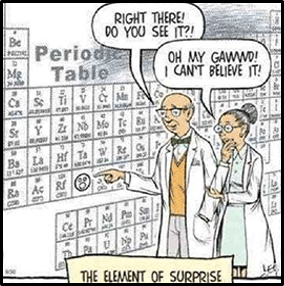
\includegraphics[width=\textwidth]{Figures/BOhBN/ah}
\end{figure}

\newpage
\chapter{Boron nitride/boron oxide as cathodes for rechargeable AIBs} 
\label{BOhBN} 

\section{Theory and background}

\begin{figure}[tbh!]
\centering
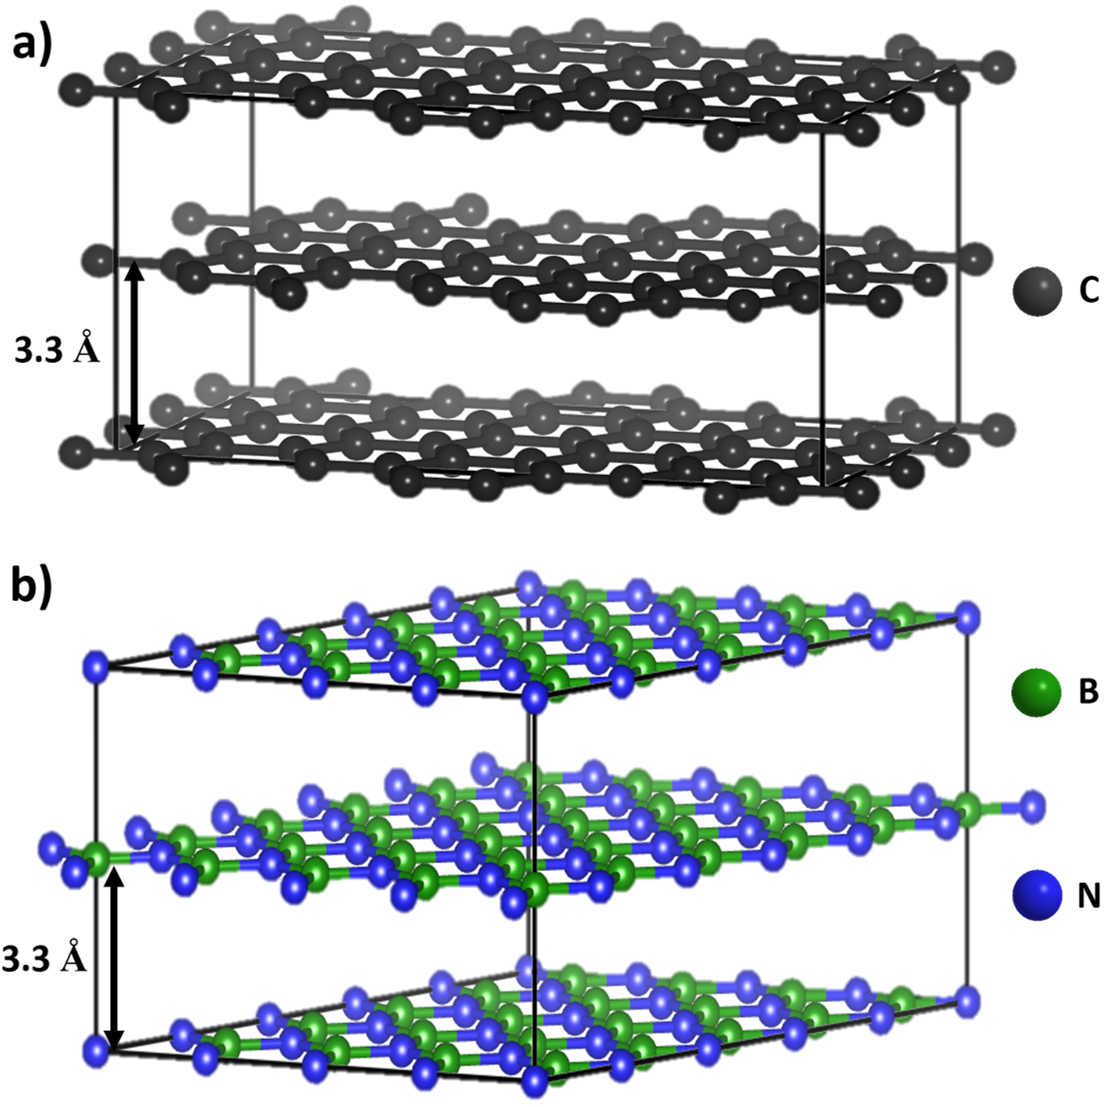
\includegraphics[width=\textwidth]{Figures/BOhBN/grpBNcomp}
\caption{Honeycomb lattice of a) natural graphite and b) hexagonal boron nitride. Both structures display an interlayer distance of 3.3\AA.}
\label{Figures/BOhBN:grpBNcomp}
\end{figure}

Graphite has been extensively used as a cathode in AIBs due to its high conductivity and a layered structure. Graphite and hexagonal boron nitride (hBN) are two prominent members of layered materials possessing a hexagonal lattice structure \cite{hod_graphite_2012}. Graphite has non-polar homonuclear C-C intralayer bonds, hBN presents highly polar B-N bonds resulting in different optimal stacking modes of the two materials in the bulk form. Furthermore, the static polarizabilities of the constituent atoms considerably differ from each other, suggesting large differences in the dispersive component of the interlayer bonding. Despite these major differences, both materials present practically identical interlayer distances, Figure \ref{Figures/BOhBN:grpBNcomp}. hBN is popularly known as "white graphene" \cite{song_large_2010, zeng_white_2010}. Structurally, a single layer of hBN is very similar to a graphene sheet having a hexagonal backbone where each couple of bonded carbon atoms is replaced by a boron nitride pair, making the two materials isoelectronic. Nevertheless, due to the electronegativity differences between the boron and the nitrogen atoms, the $\pi$ electrons tend to localize around the nitrogen atomic centers, thus forming an insulating material. The nature of bonding between nitrogen and boron differs from the carbon-carbon bonds found in graphite. hBN possesses coordinate bonds resulting from donation of \ce{e-} pair from nitrogen into empty p-orbital of a neighbouring B atom. Each N atom develops a partial positive charge and each B develops a partial negative charge. The partial ionic character of BN bonding makes it a semi-conductor as opposed to a conductor like graphite. 

\section{Results and discussion}

\begin{figure}[tbh!]
\centering
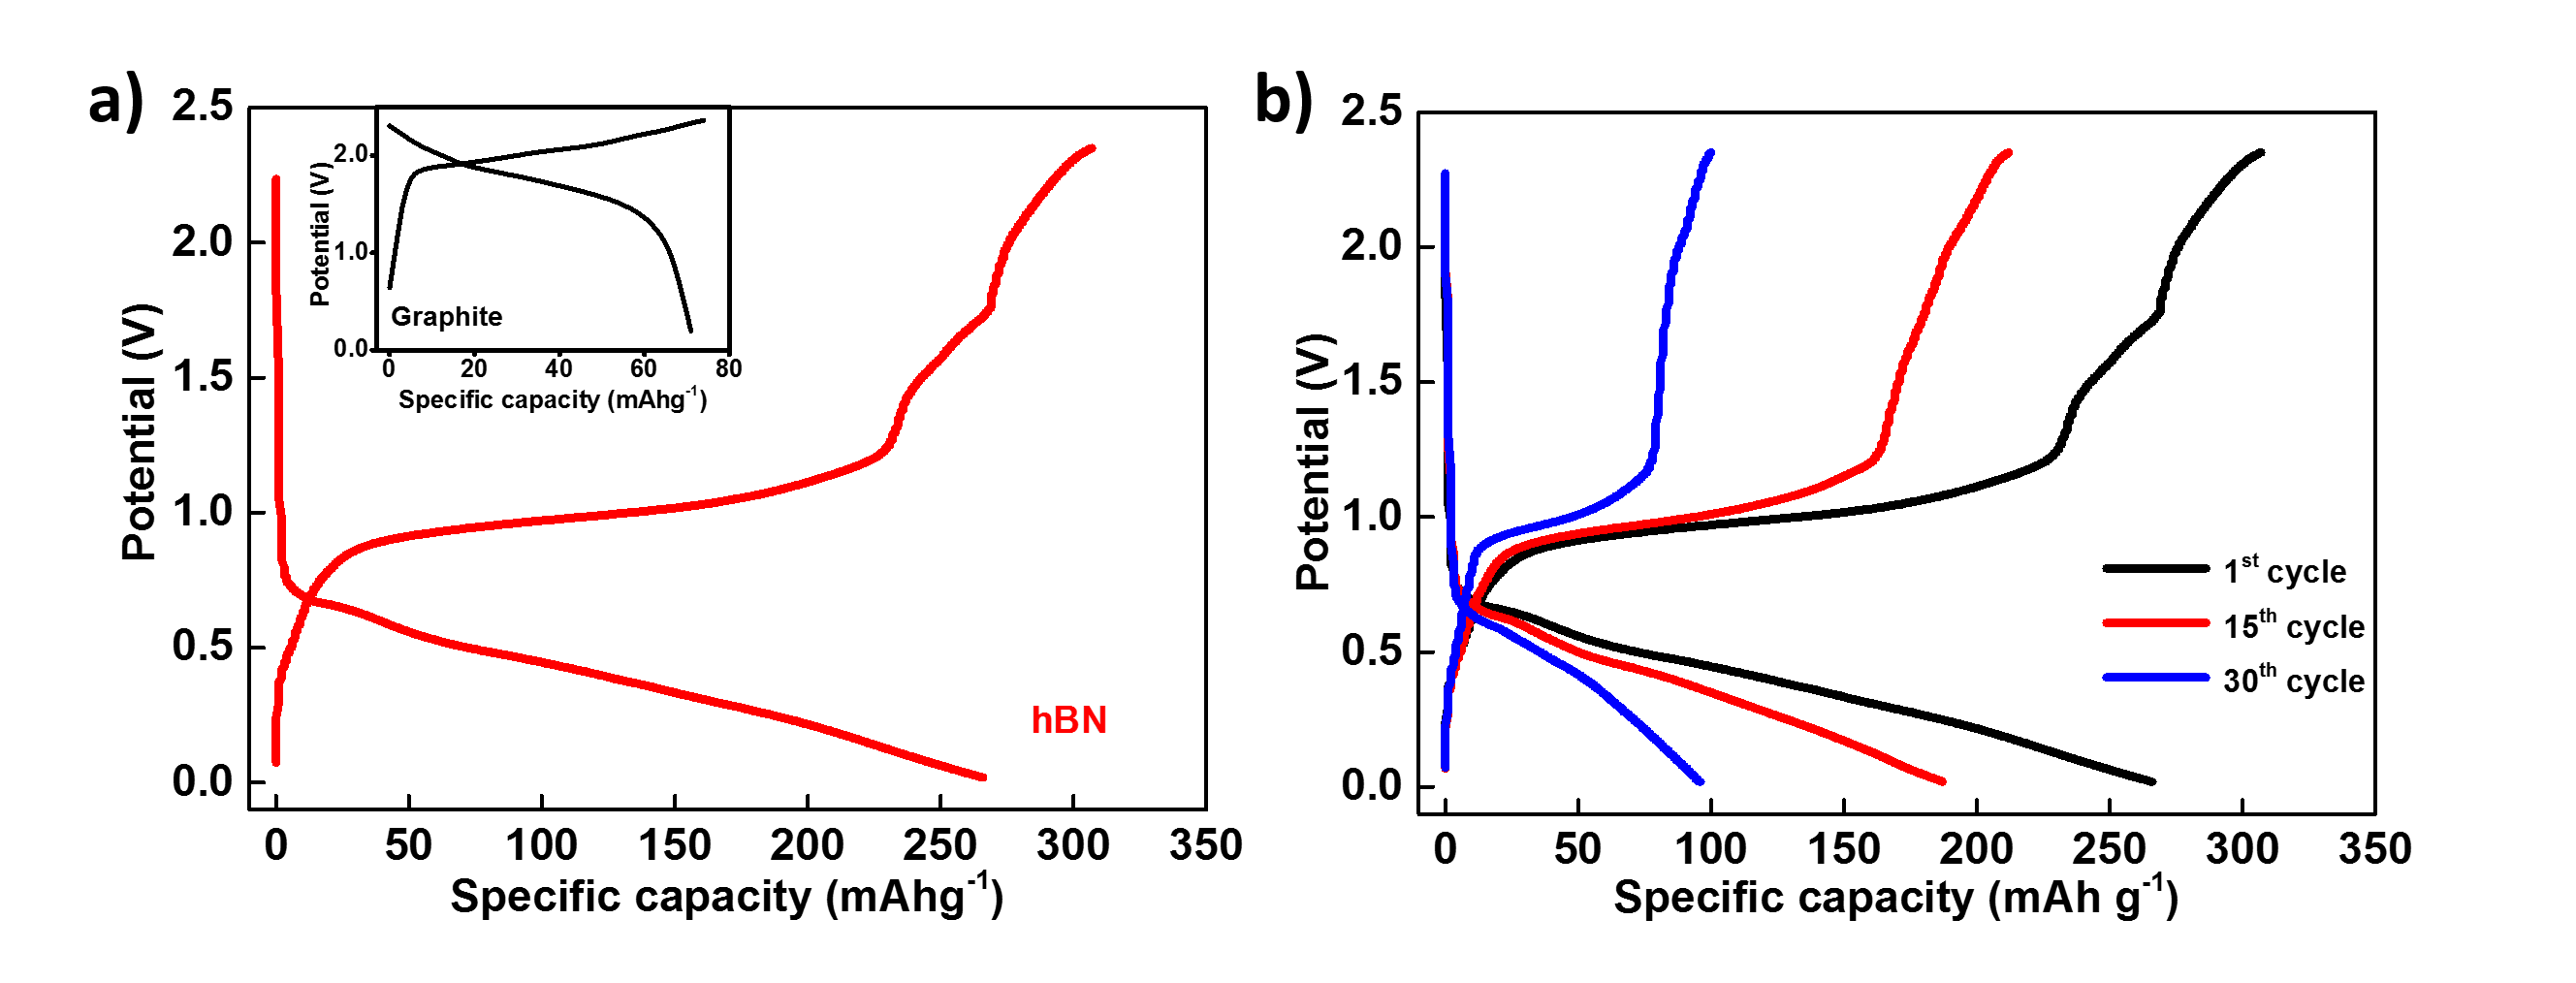
\includegraphics[width=\textwidth]{Figures/BOhBN/hBNiniCDC}
\caption{a) Galvanostatic cycles of an Al/hBN, using hBN from the stores (with \ce{B2O3} as an impurity), at a current density of 50 mA g$^{-1}$ compared with natural graphite (inset). b) Capacity fading of Al/hBN cell recorded for 30 cycles at a current rate of 50 mA g$^{-1}$.}
\label{Figures/BOhBN:hBNiniCDC}
\end{figure}

\begin{figure}[tbh!]
\centering
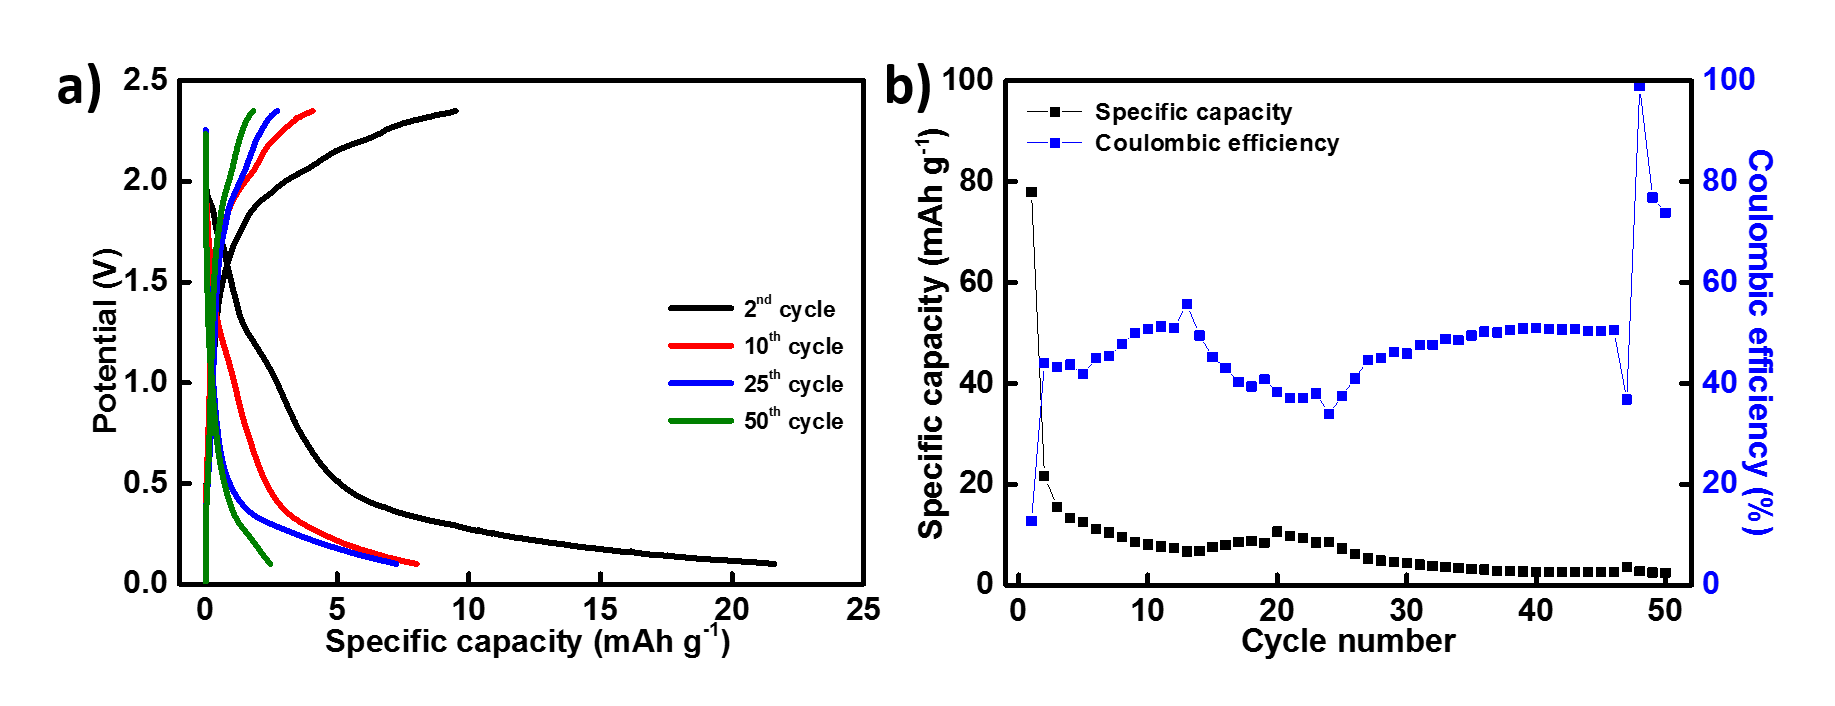
\includegraphics[width=\textwidth]{Figures/BOhBN/BNNSCDCCE}
\caption{a) Performance of an aluminium-ion battery using pure hBN as cathode at a current rate of 50 mA g$^{-1}$. b) Discharge capacity drops down to 5 mAh g$^{-1}$ after 50 cycles. hBN displays a very low coulombic efficiency $\approx$ 55\%.}
\label{Figures/BOhBN:hBNCDCCE}
\end{figure}

For all the above mentioned reasons, we tested hBN as a cathode for AIBs. To save cost, an old bottle of hBN was retrieved from VUW's chemical stores. A cell was assembled and preliminary electrochemical tests were performed. Figure \ref{Figures/BOhBN:hBNiniCDC} displays the galvanostatic charge/discharge profile of an Al/hBN cell at a current density of 50 mA g$^{-1}$. hBN exhibited very high specific capacities for the first 30 cycles of 270 mAh g$^{-1}$, which decreased to 100 mAh g$^{-1}$. The cell displayed a discharge potential of 0.6 V. Despite being not as conductive as graphite, the discharge capacity value was almost 3 times more than that of graphite (inset, Figure \ref{Figures/BOhBN:hBNiniCDC}a). Repeated measurements of Al/hBN cells using the same old bottle of hBN gave similar results, Figure \ref{Figures/appendix:hBNrepeat}. However, it was noted that the specific capacity dropped after a few cycles. In Figure \ref{Figures/BOhBN:hBNiniCDC}b, it was observed that the capacity retention of hBN was very poor (decreased by 60\%) after 30 cycles. In expectation of better results, a new bottle of hBN from Sigma Aldrich (98\%, $\sim$1 $\mu$m in size). New batch of cathodes were made and tested but surprisingly, the discharge capacity was nowhere near the older cells as displayed in Figure \ref{Figures/BOhBN:hBNCDCCE}. Many more batches were made from the new bottle and none of the cells achieved capacities higher than 50 mAh g$^{-1}$ (Figure \ref{Figures/appendix:hBNmultiattempts}! 
It was important to investigate the difference between the old and new boron nitride.

\begin{figure}[tbh!]
\centering
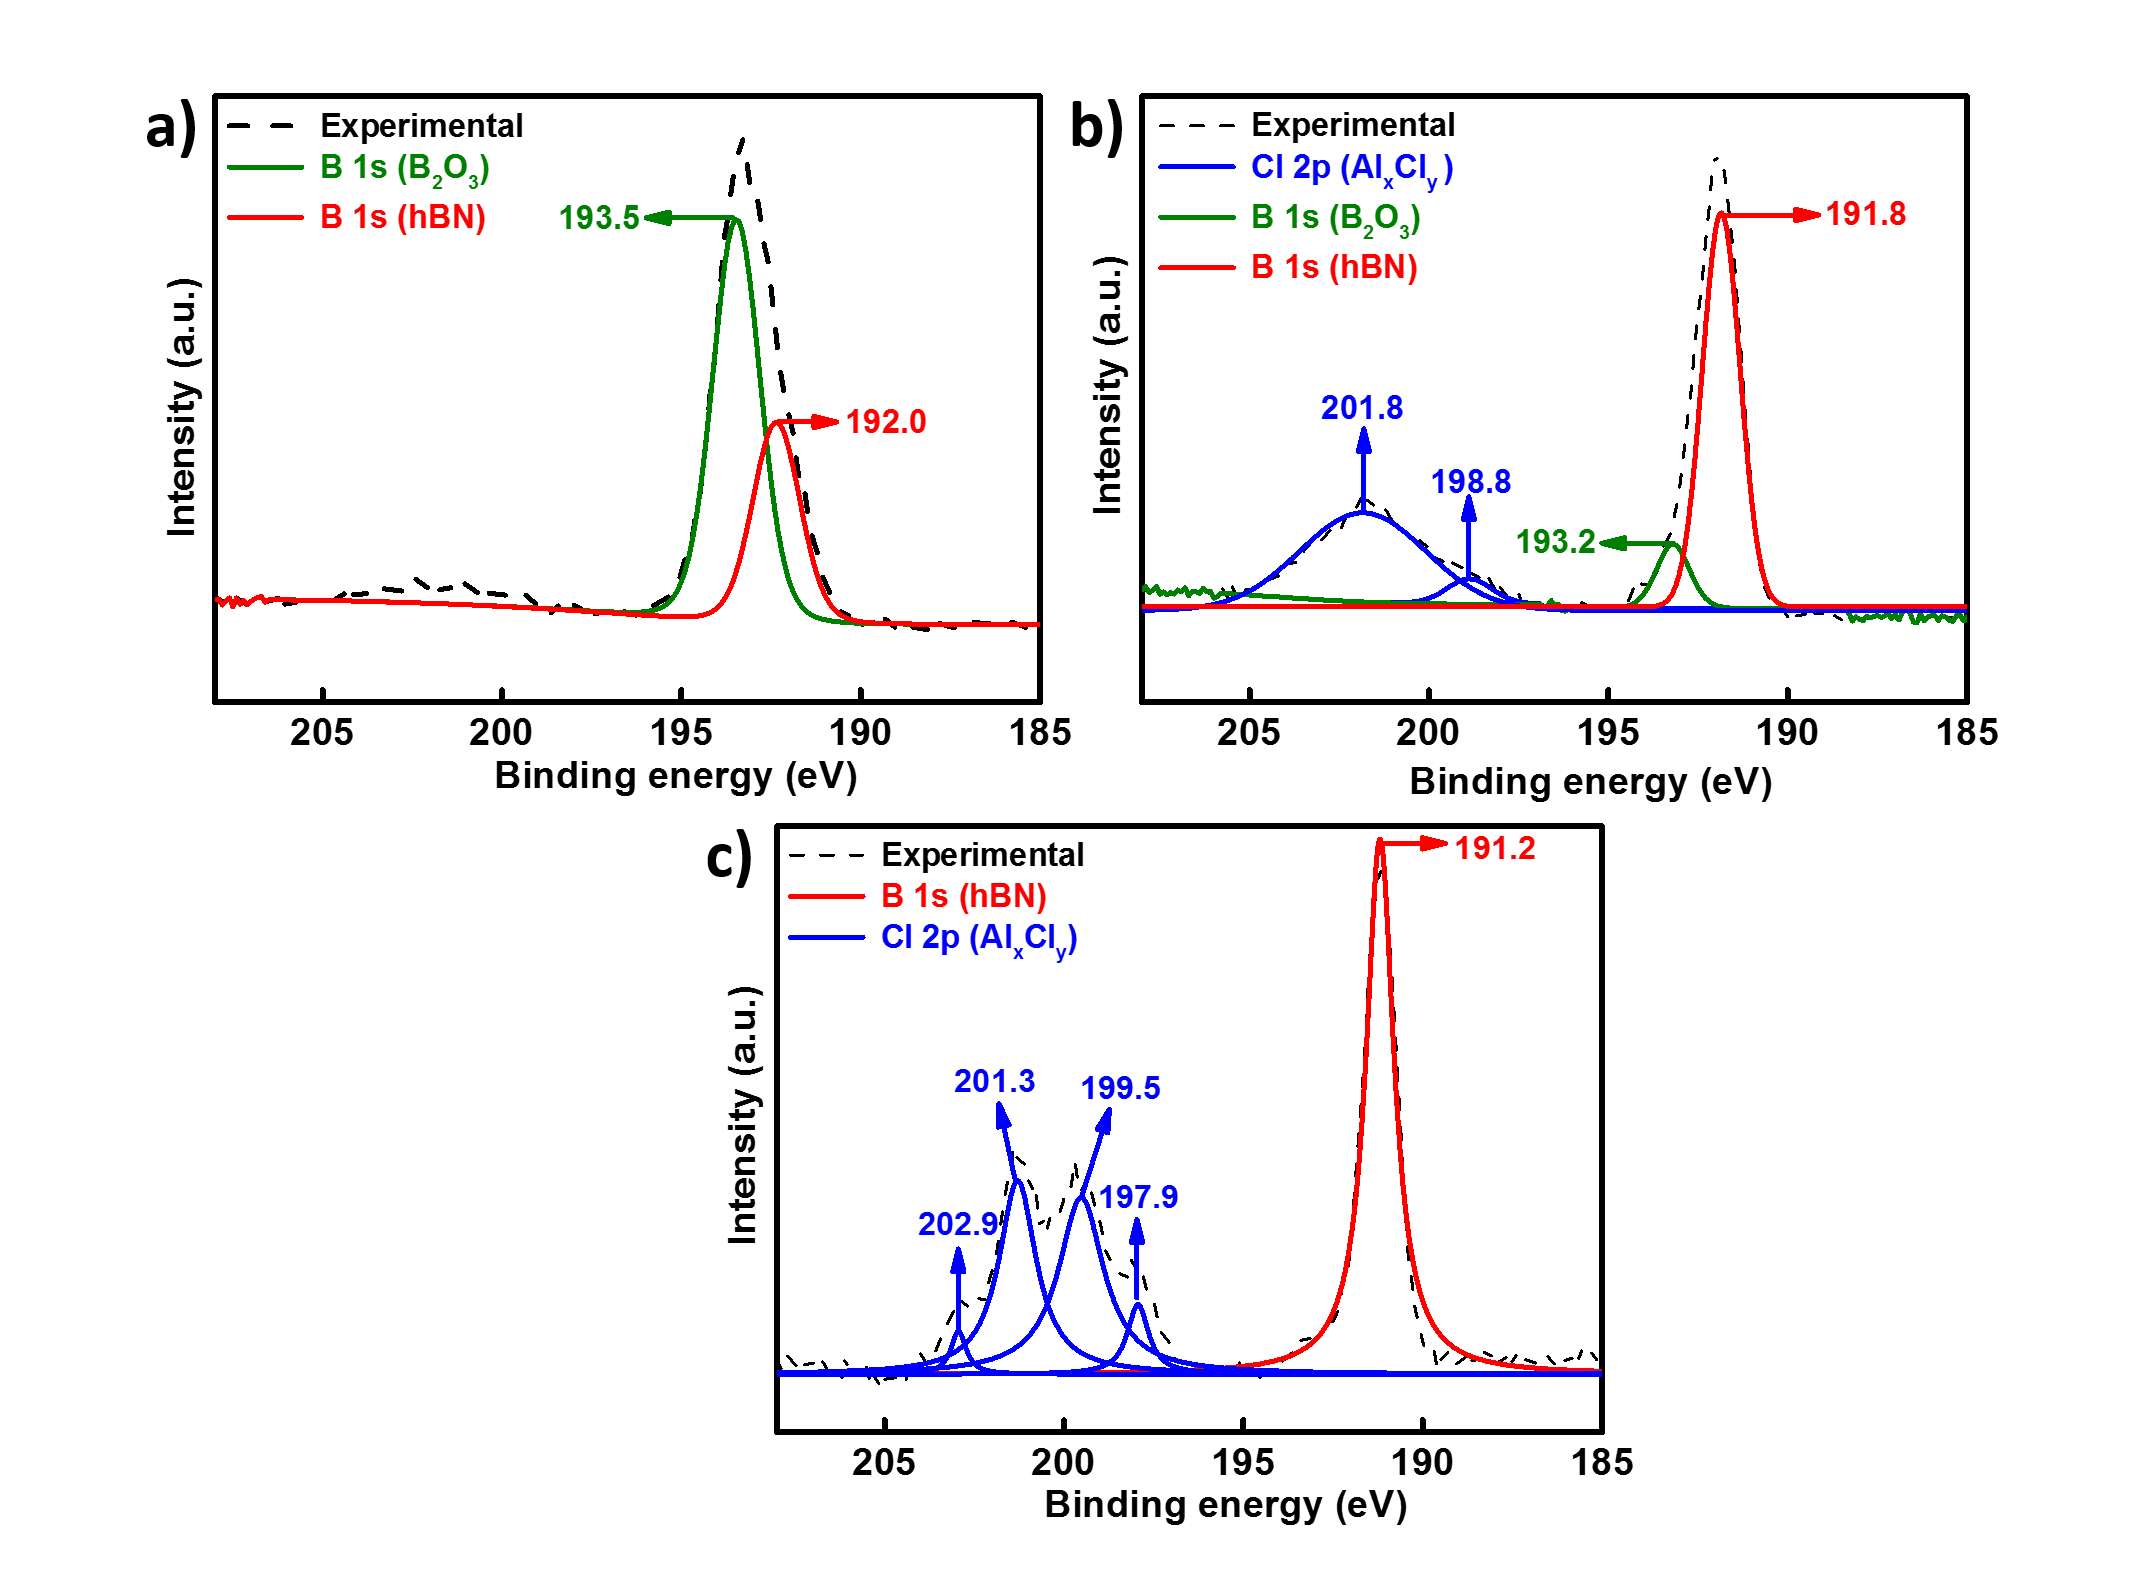
\includegraphics[width=\textwidth]{Figures/BOhBN/oldhBNXPS}
\caption{XPS spectra of a a) pristine, b) charged and c) discharges old hBN cathodes after 30 cycles.}
\label{Figures/BOhBN:oldhBNXPS}
\end{figure}

\textit{Ex-situ} X-ray photoelectron spectroscopy (XPS) of old hBN cathodes was carried out to observe the presence of various elements and the high resolution spectra obtained is shown in Figure \ref{Figures/BOhBN:oldhBNXPS}a-c). The three spectra reveal the presence of B and Cl elements for a pristine (Figure \ref{Figures/BOhBN:oldhBNXPS}a) charged (Figure \ref{Figures/BOhBN:oldhBNXPS}b) and discharged (Figure \ref{Figures/BOhBN:oldhBNXPS}c) cathode. Cl 2p binding energy is absent in the spectra of the pristine electrode, which was without any contact with the electrolyte, and was dominated by the B-O and B-N peaks. Presence of \ce{B2O3} would result in B-O bonds, which is what is observed in Figure \ref{Figures/BOhBN:oldhBNXPS}a. The presence of Cl in the charged and discharged cathodes is mainly derived from electrolyte contamination. It can been seen from Figure \ref{Figures/BOhBN:oldhBNXPS}a-c) that the binding energy of B 1s includes a pair of peaks at 193.5 and 192.0 eV before test, which are attributed to B-O (from \ce{B2O3}) and B-N bonds (from hBN) respectively. After discharging to 0.3 V, the B-O bond completely disappears as shown in Figure \ref{Figures/BOhBN:oldhBNXPS}c. Cl 2p binding energy at 201.8 and 198.8 eV separates into four peaks at 202.9, 201.3, 199.5 and 197.9 eV. The binding energies (charged cathode) at 193.2 and 191.8 eV are again attributed to B-O from \ce{B2O3} and B-N from hBN respectively. After complete discharge, the B-O bond's binding energy is completely eliminated and only B-N bond remains.

\begin{figure}[tbh!]
\centering
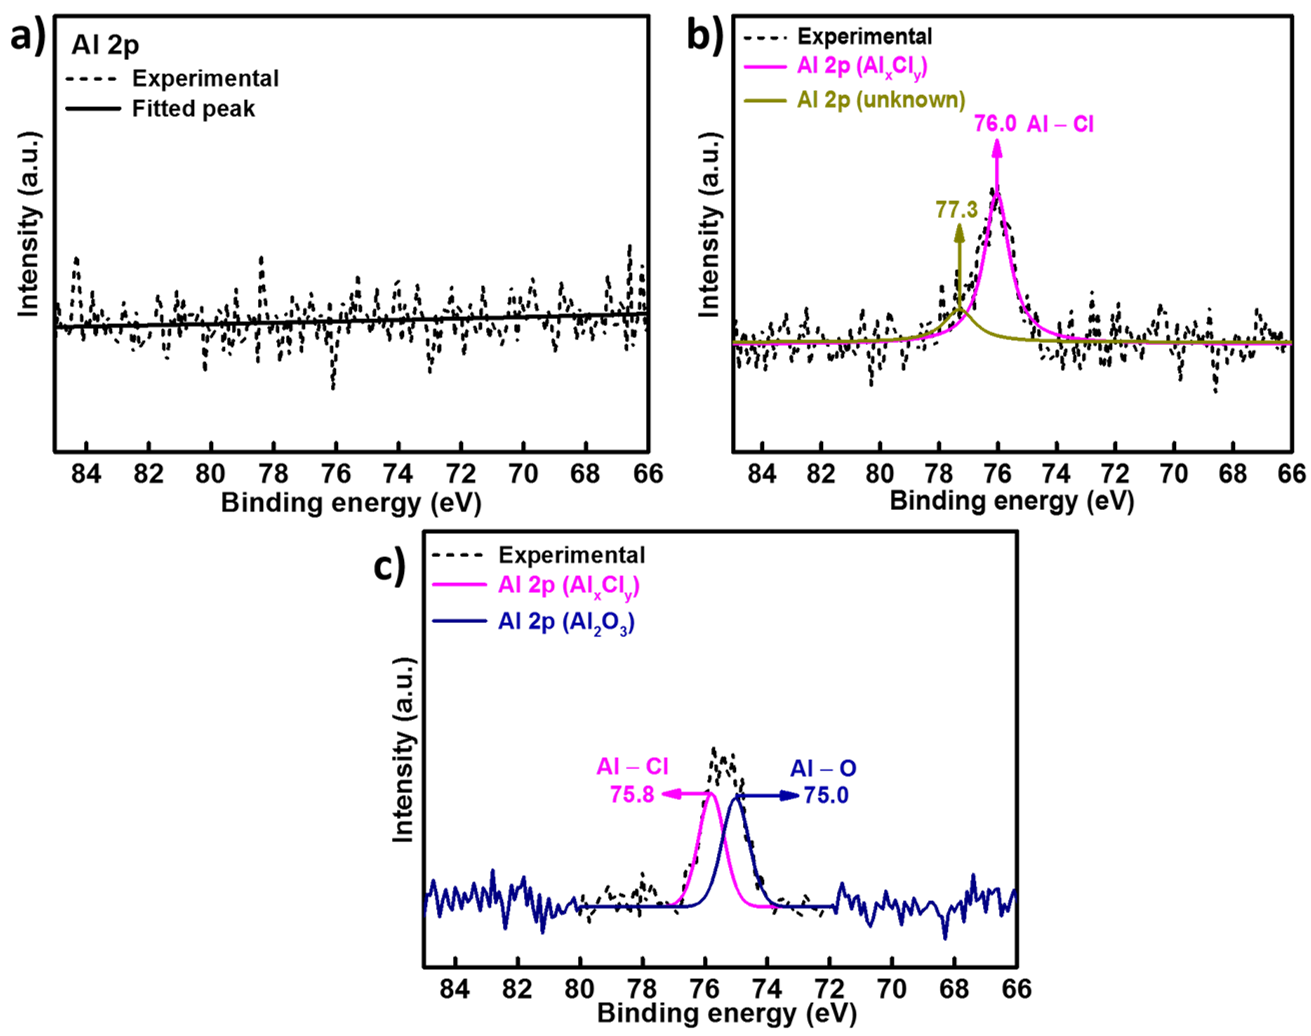
\includegraphics[width=\textwidth]{Figures/BOhBN/hBNAlXPS}
\caption{Honeycomb lattice of a) natural graphite and b) hexagonal boron nitride. Both structures display an interlayer distance of 3.3\AA.}
\label{Figures/BOhBN:hBNAlXPS}
\end{figure}

XPS results of the of Al 2p orbital confirm variation of the Al valence during cell charge and discharge. During cell charging (Figure \ref{Figures/BOhBN:hBNAlXPS}b), the Al 2p peak deconvolutes into two binding energies at 76.0 and 77.3 eV. The peak at 76.0 eV can be attributed to Al-Cl bond from the chloroaluminates (\ce{AlxCly}). After complete discharge (Figure \ref{Figures/BOhBN:hBNAlXPS}c), the peak further splits into two binding energies at 75.0 and 75.8 eV. The binding energy at 75.0 eV can be attributed to an Al-O bond from possible formation of \ce{Al2O3} during discharge and the energy at 75.8 eV corresponds to chloroaluminates. If the electronegativity of the doping element is higher than Al, the electron density around Al decreases and its binding energy increases. Chlorine has a higher electronegativity than oxygen, therefore the peak at higher binding energy is attributed to \ce{AlxCly} and lower corresponds to \ce{Al2O3}. Since the pristine cathode was untouched from the electrolyte, no spectra was observed in Figure \ref{Figures/BOhBN:hBNAlXPS}a. It was to be noted that the binding energy of Al 2p in the oxidized state is 75 eV, very close to a typical Al in \ce{Al2O3} at 74.5 eV \cite{}. 

\begin{figure}[tbh!]
\centering
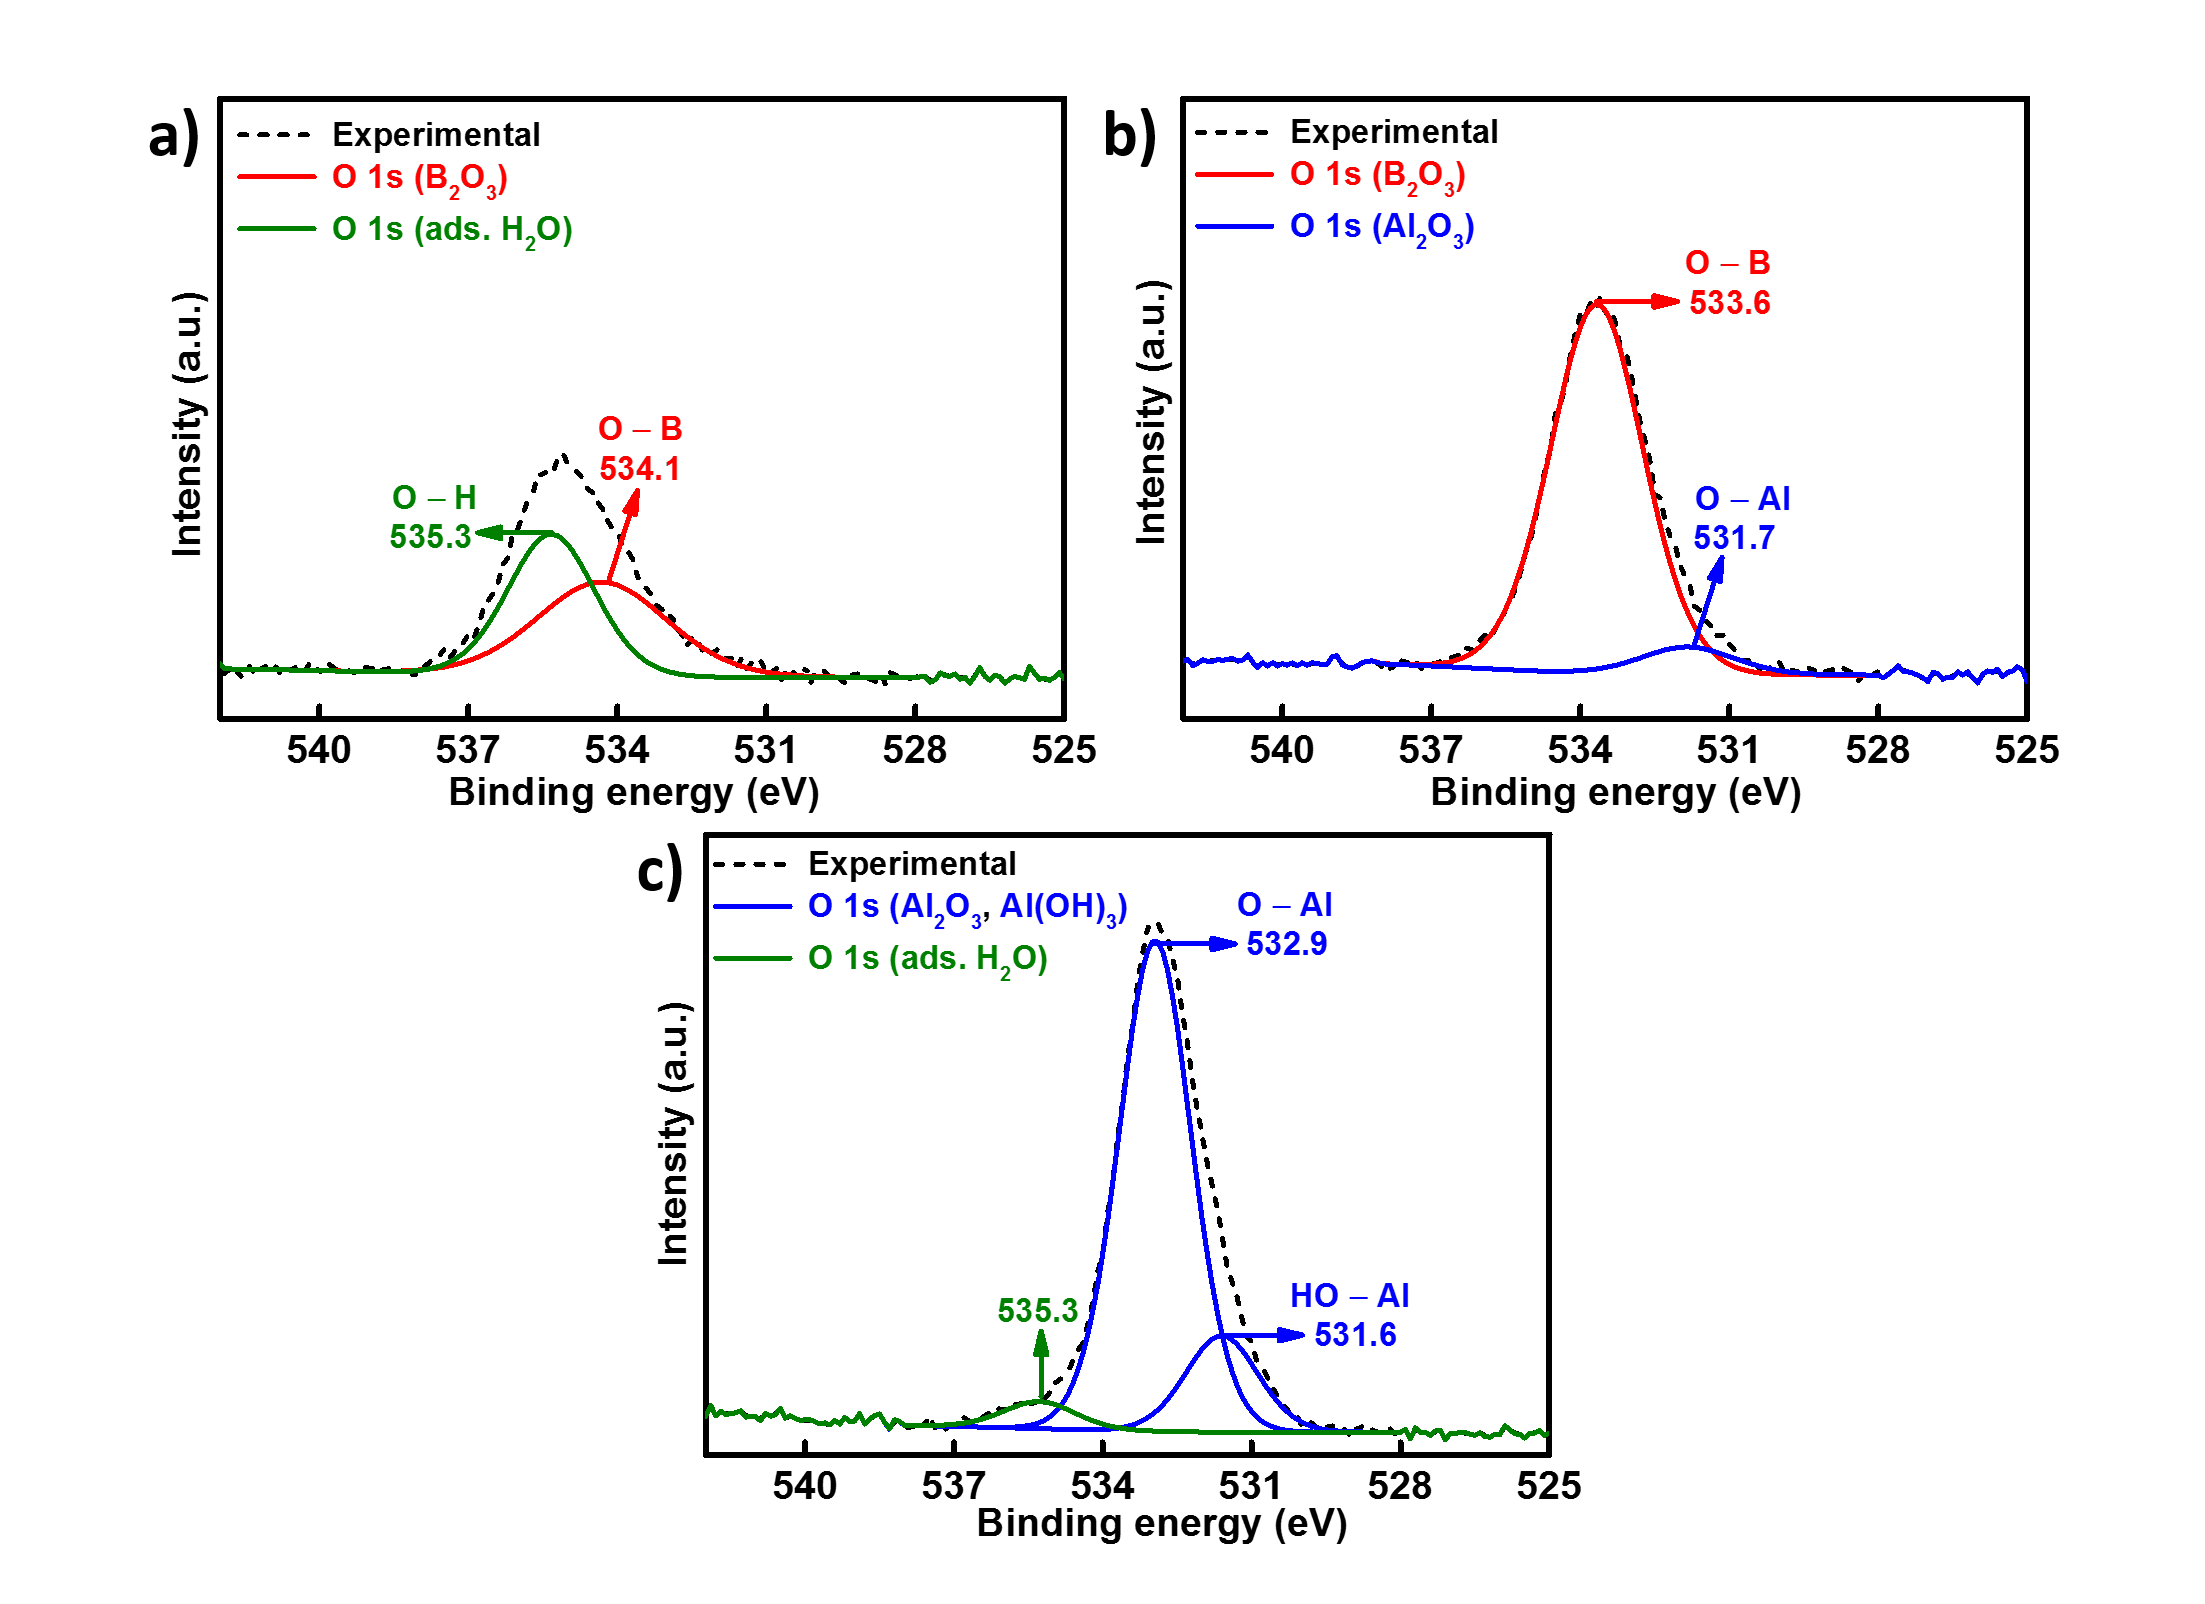
\includegraphics[width=\textwidth]{Figures/BOhBN/hBNOXPS}
\caption{Honeycomb lattice of a) natural graphite and b) hexagonal boron nitride. Both structures display an interlayer distance of 3.3\AA.}
\label{Figures/BOhBN:hBNOXPS}
\end{figure}

Figure \ref{Figures/BOhBN:hBNOXPS}a-c) shows the high resolution O 1s spectra of the pristine (Figure \ref{Figures/BOhBN:hBNOXPS}a), charged (Figure \ref{Figures/BOhBN:hBNOXPS}b) and discharged (Figure \ref{Figures/BOhBN:hBNOXPS} cathodes. The O 1s core level spectrum for pristine hBN (Figure \ref{Figures/BOhBN:hBNOXPS}a) can be deconvoluted into two peaks that corresponds to an O-H bond (at 535.3 eV), which comes from adsorbed moisture from the environment. From the deconvoluted spectrum, binding energy from an O-B bond appears at 534.1 eV, which confirms presence of \ce{B2O3} in the old hBN sample. In the charged cathode, the major contribution comes from \ce{B2O3} (92\%) at 533.6 eV and the remaining 8\% from O-Al with a peak at 531.7 eV, suggesting presence of \ce{Al2O3}.  Figure \ref{Figures/BOhBN:hBNOXPS}c shows the spectrum after complete discharge. The peak obtained was deconvoluted into three binding energies at 535.3, 532.9 and 531.6 eV, corresponding to an O-H bond from adsorbed moisture, O-Al and OH-Al bonds from \ce{Al2O3} and possible formation of \ce{Al(OH)3} \cite{}. From XPS analysis the results strongly indicate:

\begin{itemize}
\item presence of \ce{B2O3} in the pristine hBN sample, which disappears after discharge and comes back after charge
\item formation of \ce{Al2O3} during cycles, with a strong presence after complete discharge. Some chloroaluminates remain in the sample after cycling and for this reason, Al-O bond appears in both charged and discharged cathodes.
\end{itemize} 

XPS analysis was immensely helpful in hypothesising the mechanism of an Al/hBN/\ce{B2O3} cell. The following reaction supposedly takes place during discharge:

\begin{equation}
    0.5\ce{B2O3 + AlCl3 + 3e-} \longrightarrow \ce{B + 0.5Al2O3 + 3Cl-}
\end{equation}

\begin{figure}[tbh!]
\centering
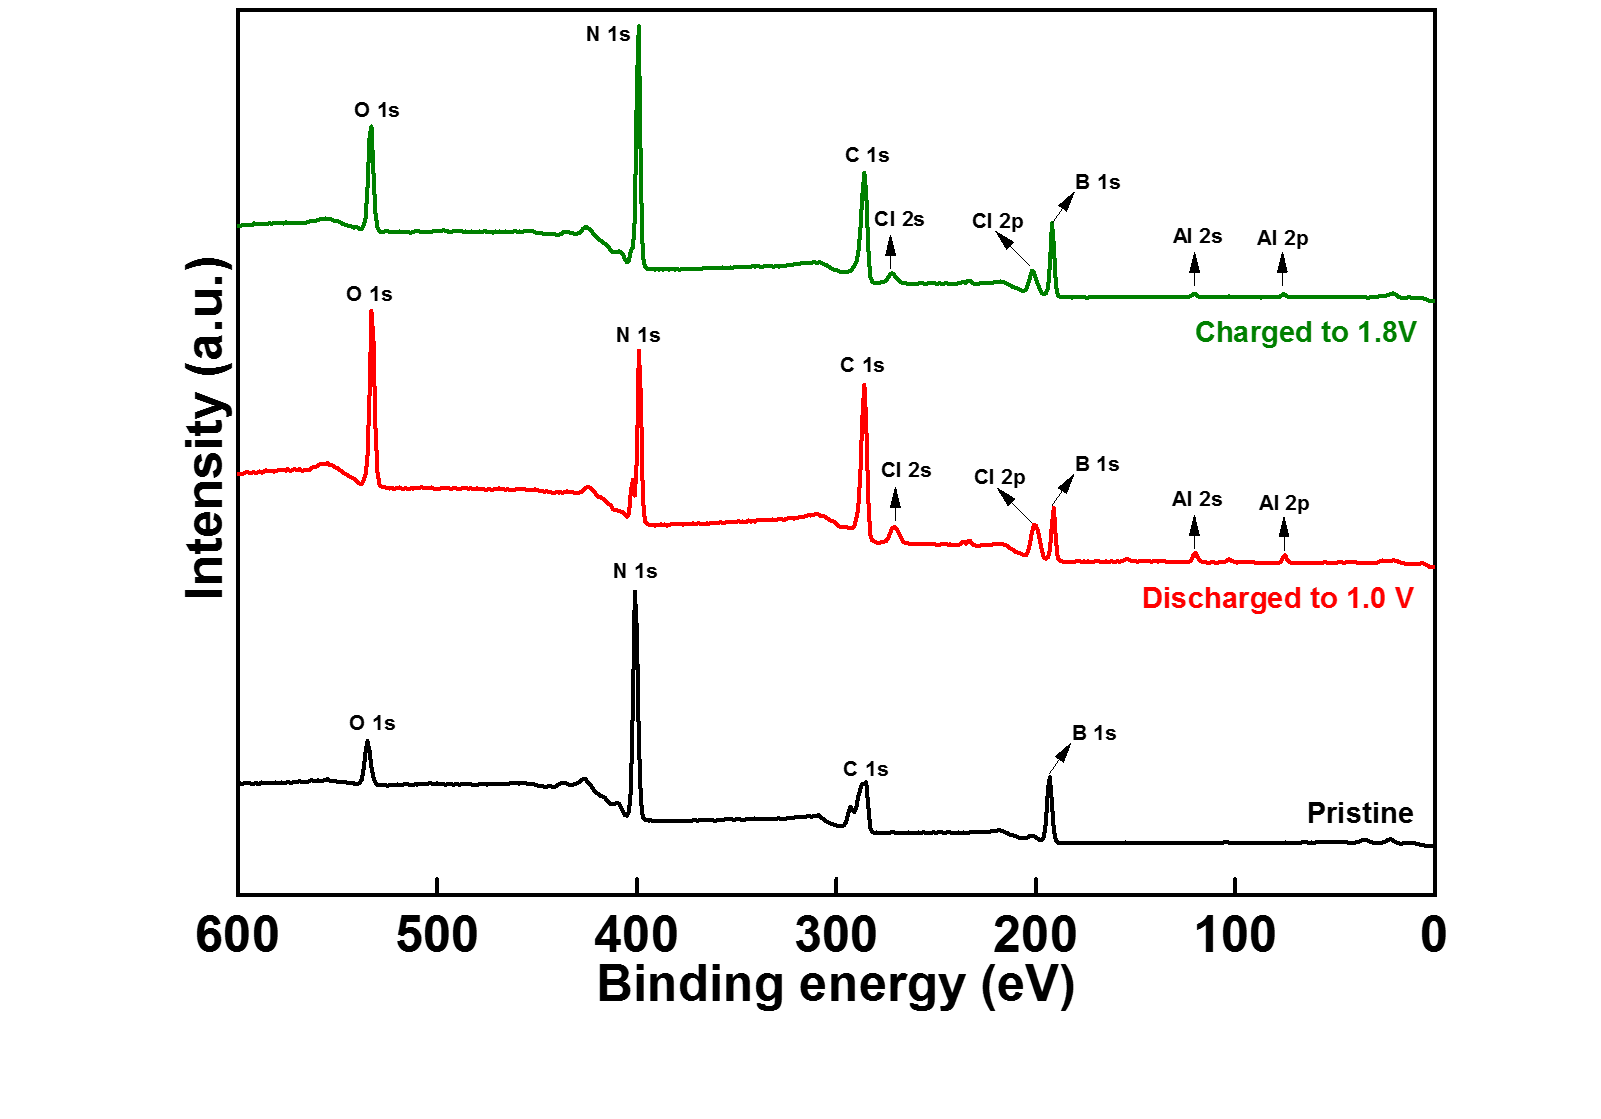
\includegraphics[width=\textwidth]{Figures/BOhBN/hBNXPS}
\caption{A wide scan spectrum of pristine (in black), discharged (in red) and charged (in green) hBN (old) cathode. Figure shows the survey spectra with peaks corresponding to aluminum and chlorine observed in the charged and discharged cathodes. Intensity of Al 2p and Cl 2p is higher in discharged cathode.}
\label{Figures/BOhBN:hBNXPS}
\end{figure}

\begin{figure}[tbh!]
\centering
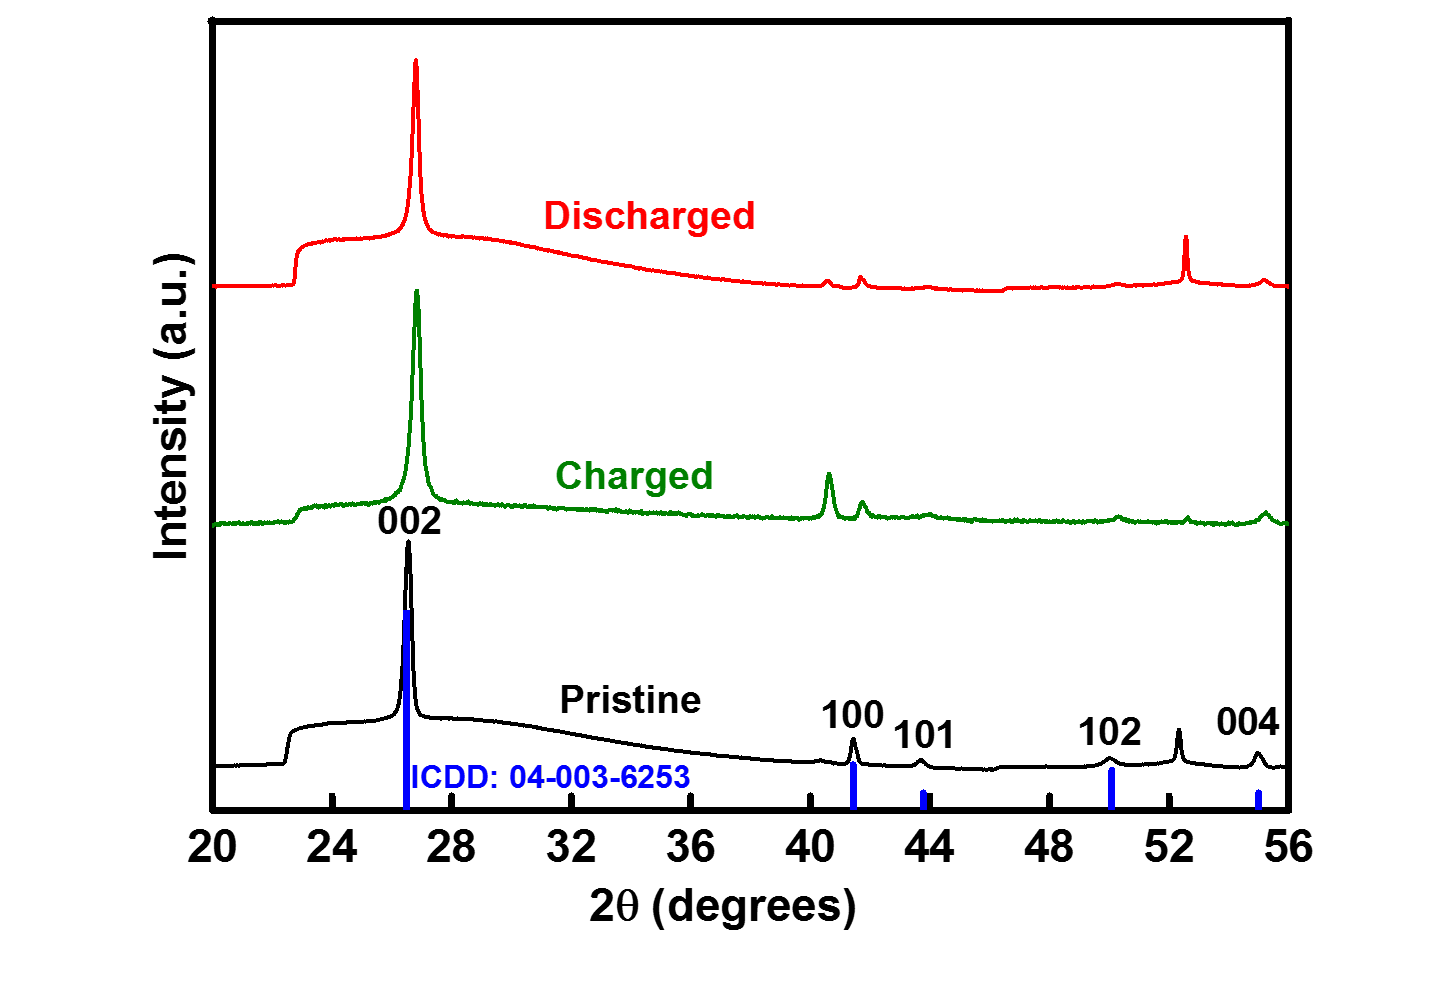
\includegraphics[width=\textwidth]{Figures/BOhBN/hBNXRD2}
\caption{.}
\label{Figures/BOhBN:hBNXRD2}
\end{figure}

In Figure \ref{Figures/BOhBN:hBNXRD2} X-ray diffraction patterns of pristine (in black), charged (in green) and discharged (in red) cathodes is shown. The patterns are in good agreement with the standard ICDD pattern (04-003-6253) and show the existence of hexagonal boron nitride with P6/mmc space group. The miller indices (hkl) of all the characteristic peaks are marked as per the standard pattern. The characteristic peak at 2$\theta$ value of 26.5$^{\circ}$ confirms a d-spacing of 3.3\AA\. The presence of an amorphous peak is suggestive towards the presence of \ce{B2O3}. Interestingly, a new peak is observed at a 2$\theta$ value of 52.36$^{\circ}$. This newly formed peak possibly corresponds to \ce{B2O3} of a trigonal structure. In addition, there is a small change in the lattice parameters due to the slight shift observed for some peaks as shown in Figure \ref{Figures/BOhBN:hBNXRD2} during the charge and discharge process. This corresponds to a change in the lattice structure of the host material. 

\textit{Ex-situ} SEM experiments were conducted to determine the structural changes taking place in the old hBN cathode. The structural change in the electrode after 30 charge/discharge cycles is shown in Figure \ref{Figures/BOhBN:hBNSEM} a-d). The pristine cathodes (Figure \ref{Figures/BOhBN:hBNSEM} a and c display the typical hexagonal shaped boron nitride. Figure \ref{Figures/BOhBN:hBNSEM} b and d confirm a change in cathode morphology and showed agglomeration. This could be possibly why the capacity starts to fade after a few cycles.

\begin{figure}[tbh!]
\centering
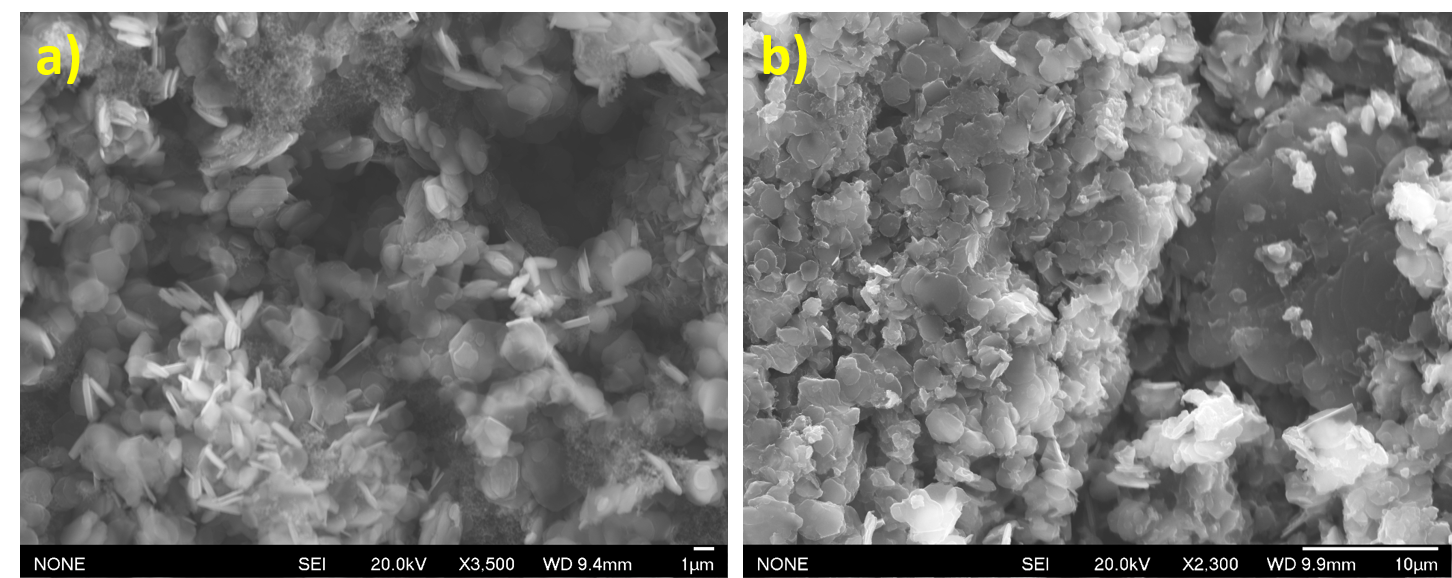
\includegraphics[width=\textwidth]{Figures/BOhBN/hBNSEM}
\caption{SEM images of a), c) pristine hBN. The hexagonal shape of boron nitride is distinctly visible. Figure\ref{Figures/BOhBN:hBNSEM} b and d) suggest that after a few cycles, the particles agglomerate. The particles retain their distinct hexagonal shape.}
\label{Figures/BOhBN:hBNSEM}
\end{figure}

\section*{Boron nitride nano sheets (BNNS)}
As mentioned in previous chapters, nano-sized materials increase the contact area between an electrode and electrolyte. They provide short path lengths for both ion diffusion and electron transport, which improves the charge/ discharge rate. The high surface area of the material allows large volume expansion/ contraction associated with ion transport and prevents cathode pulverisation leading to longer cycle-life \cite{zhang_ultrathin_2015,  cong_intrinsic_2015}. 
In expectation of better results, nano sheets of hexagonal boron nitride were synthesised via mechanical exfoliation.
250 mg of hBN was dispersed in 75 ml isopropanol (IPA) in a 100 ml round bottom flask (RBF). The mixture was heated at 500$^{\circ}$C for 24 hours and was magnetically stirred. To accelerate the dissolution of hBN into IPA, the RBF was then put in an ultrasonic bath for 20 hours. The solution was then left to stand for 2 days and the supernatant was removed in a centrifuge tube. It was centrifuged at a speed of 14000 rpm. The obtained precipitate was washed with acetone to remove residual IPA. The product was dried overnight at 60$^{\circ}$C. 

\begin{figure}[tbh!]
\centering
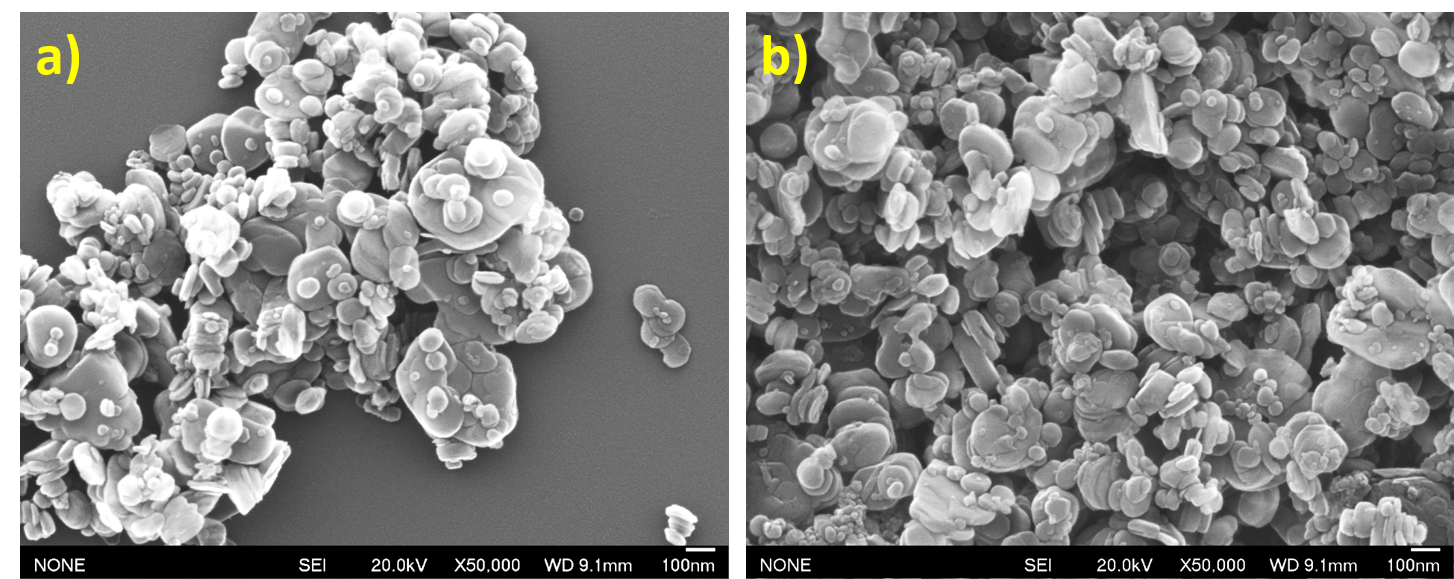
\includegraphics[width=\textwidth]{Figures/BOhBN/BNNSSEM}
\caption{SEM images of hexagonal boron nitride nano sheets.}
\label{Figures/BOhBN:BNNSSEM}
\end{figure}

Cathodes for aluminium-ion batteries were made using BNNS and the galvanostatic charge/discharge profile is displayed in Figure \ref{Figures/BOhBN:BNNSCDCCE}a and b. Capacity fade was similar to what was observed in hBN and so was the low coulombic efficiency. This experiment proved that hBN was indeed not an active material at all and the capacity came from \ce{B2O3}. 

\begin{figure}[tbh!]
\centering
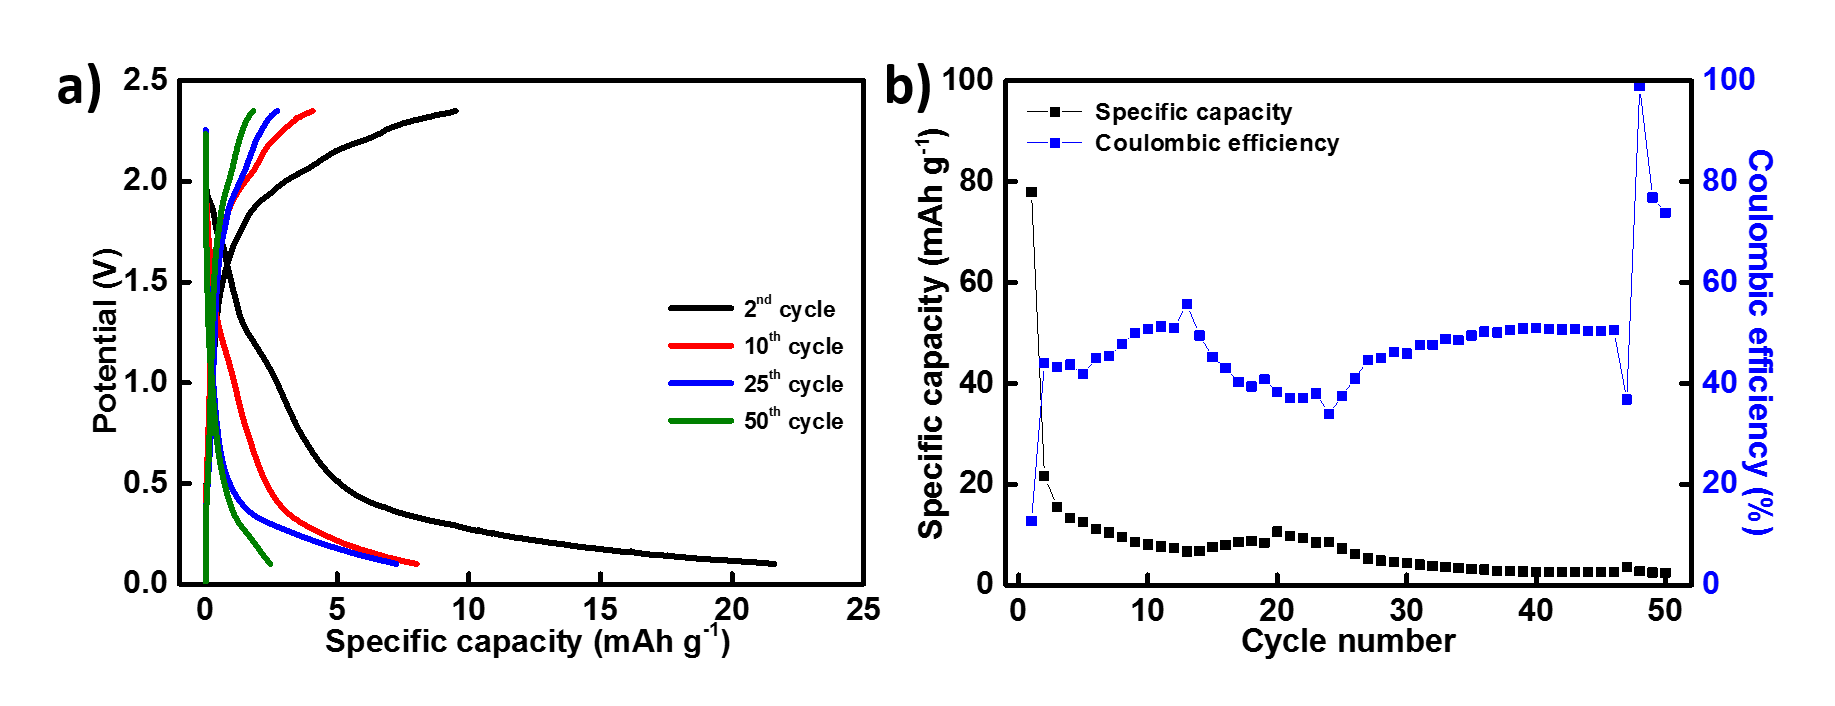
\includegraphics[width=\textwidth]{Figures/BOhBN/BNNSCDCCE}
\caption{Galvanostatic charge/discharge profile of Al/BNNS cell at a current rate of 50 mA g$^{-1}$. The cell achieved 22 mA h g$^{-1}$ in its first cycle, which dropped down to 2 mAh g$^{-1}$ after 50 cycles. Coulombic efficiency was also very low $\sim$50\%. }
\label{Figures/BOhBN:BNNSCDCCE}
\end{figure}

\section*{Boric anhydride \ce{B2O3} as an active material}
Performance of aluminium-ion cells using \ce{B2O3} as the active material in the cathode is shown in Figure \ref{Figures/BOhBN:BOCDC}. 

\begin{figure}[tbh!]
\centering
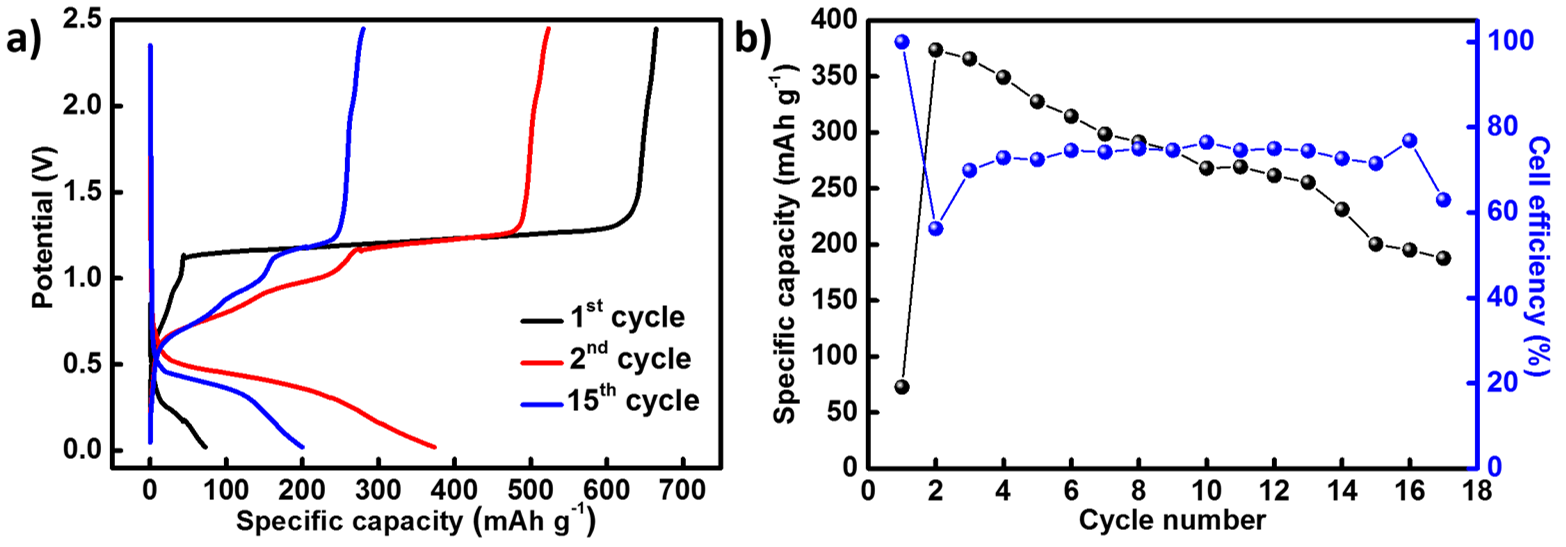
\includegraphics[width=\textwidth]{Figures/BOhBN/BOCDC}
\caption{Charge/discharge profile of pure \ce{B2O3} as the active material in an AIB at the current rate of 50 mA g$^{-1}$. After 15 cycles, the capacity drops by $\sim$50\%. Coulombic efficiency of Al/\ce{B2O3} is low and  stabilises at $\sim$78\%.}
\label{Figures/BOhBN:BOCDC}
\end{figure}

It was possible that both hBN and \ce{B2O3} were responsible for storing high specific capacity, which were observed in Figure \ref{Figures/appendix:hBNrepeat}. 

\begin{figure}[tbh!]
\centering
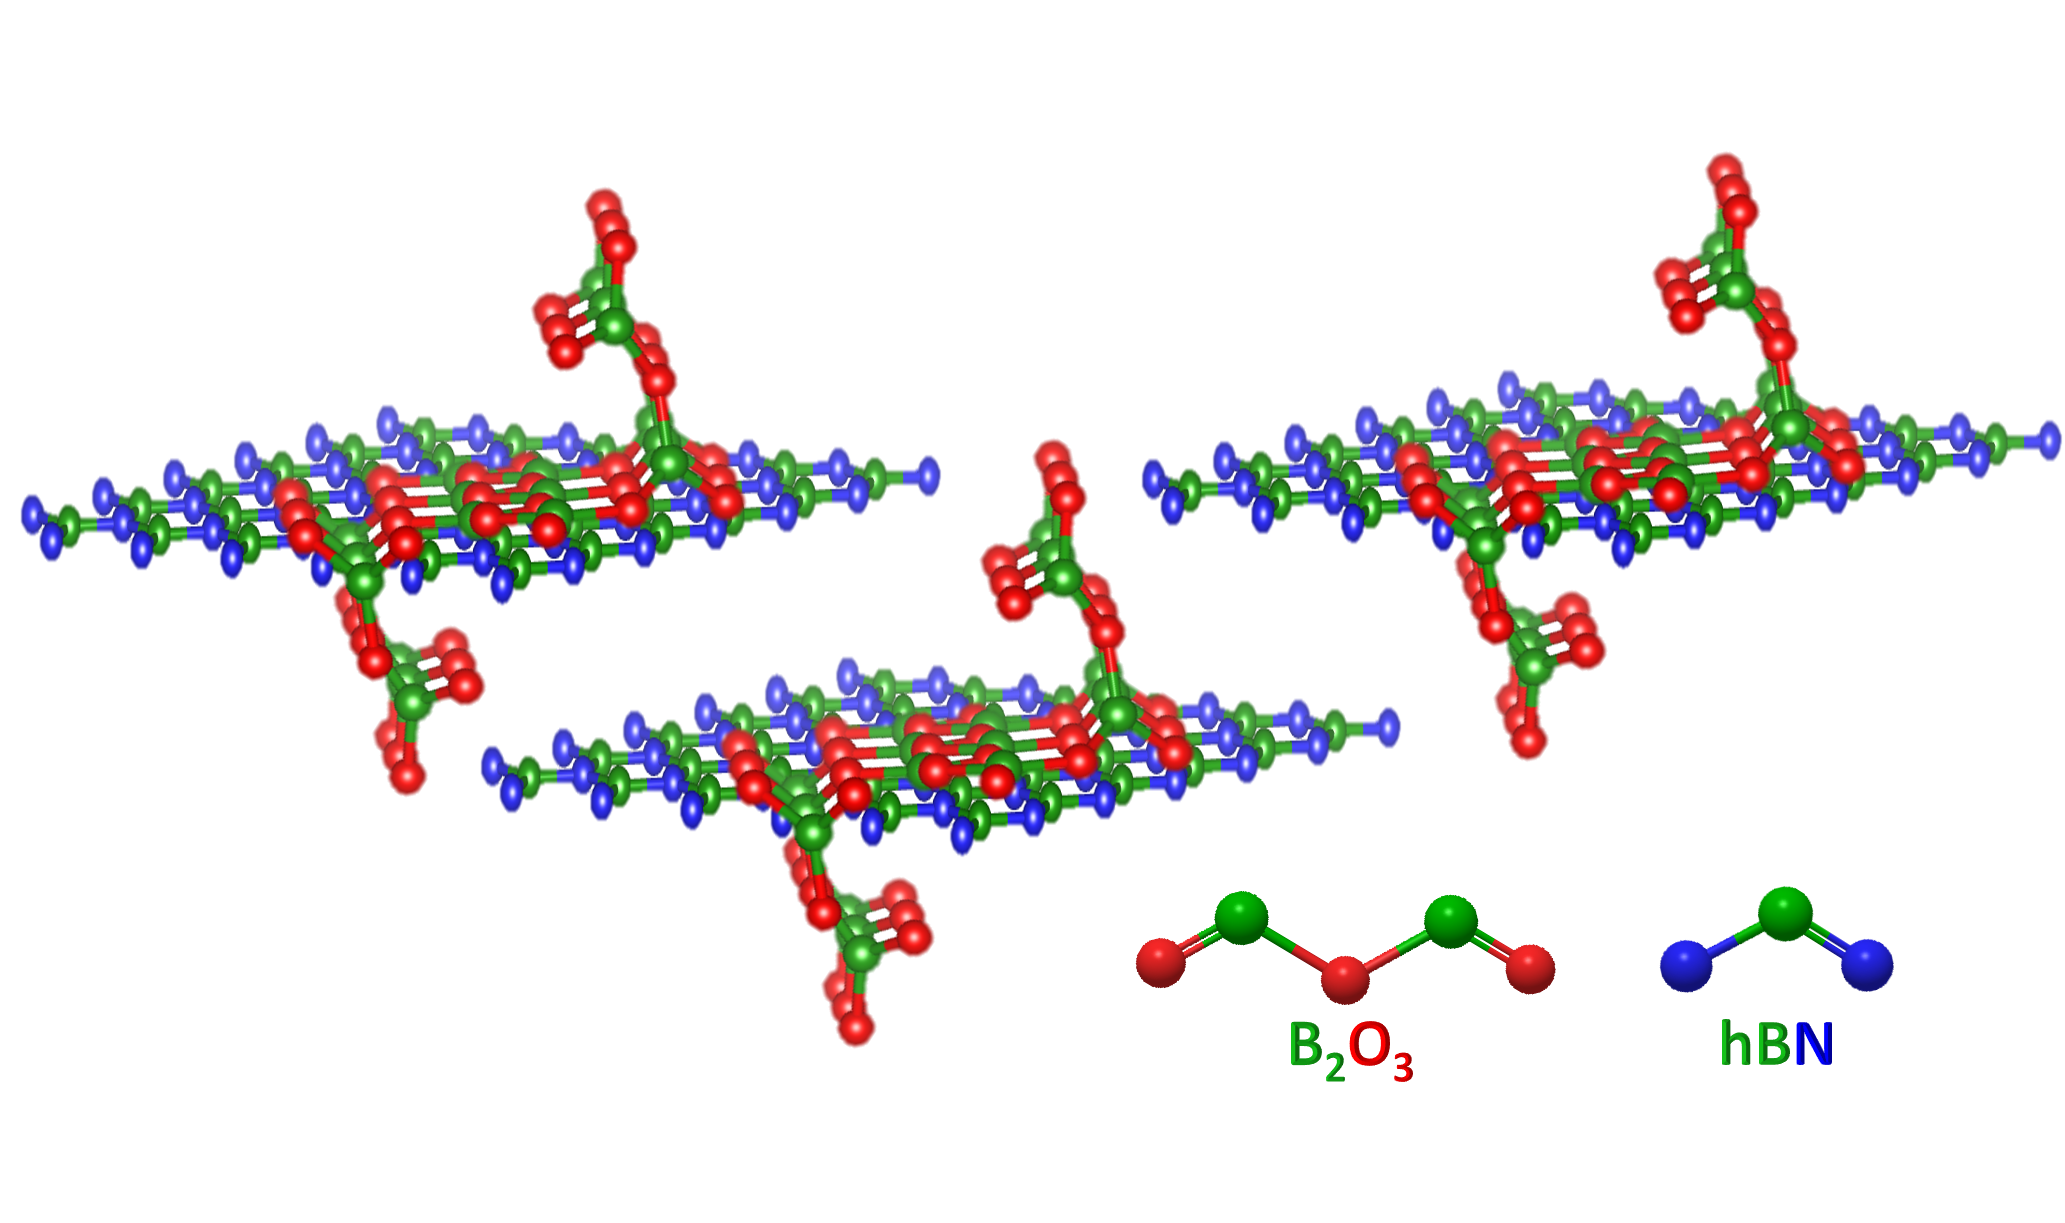
\includegraphics[width=\textwidth]{Figures/BOhBN/BonhBN}
\caption{Schematic showing the layered structure of hBN supporting \ce{B2O3}. During discharge \ce{AlCl3} reacts with \ce{B2O3} resulting in formation of elemental boron and \ce{Al2O3} and free \ce{Cl-} ions. Further analysis is needed to fully understand the role of hBN.}
\label{Figures/BOhBN:BohBN}
\end{figure}

Different weight ratios were tested to find out which one performed the best. Since the role of hBN was not established it was probable that hBN was just providing structural support to the amorphous \ce{B2O3}. The ratios and their performance is tabulated below in Table \ref{tabdiffpc}. All cells had a discharge volatge plateau at $\sim$ 0.6 V

\begin{table}[tbh!]
\centering
\caption{Comparing performance of hBN/\ce{B2O3} cathodes at different weight percentages.} \label{tabdiffpc}
\begin{tabular}{|ccc|}
\hline
\textbf{Weight \% of} & \textbf{Weight \% of} & \textbf{Discharge capacity in 20th cycle} \\
\textbf{hBN} & \textbf{\ce{B2O3}} & \textbf{mAh g$^{-1}$} \\
\hline
\hline
25 & 75 & 22\\
20 & 80 & 48\\
15 & 85 & 48\\
10 & 90 & 68\\
5 & 95 & 171\\
0 & 100 & 104\\
\hline 
\end{tabular}
\end{table}

\begin{figure}[tbh!]
\centering
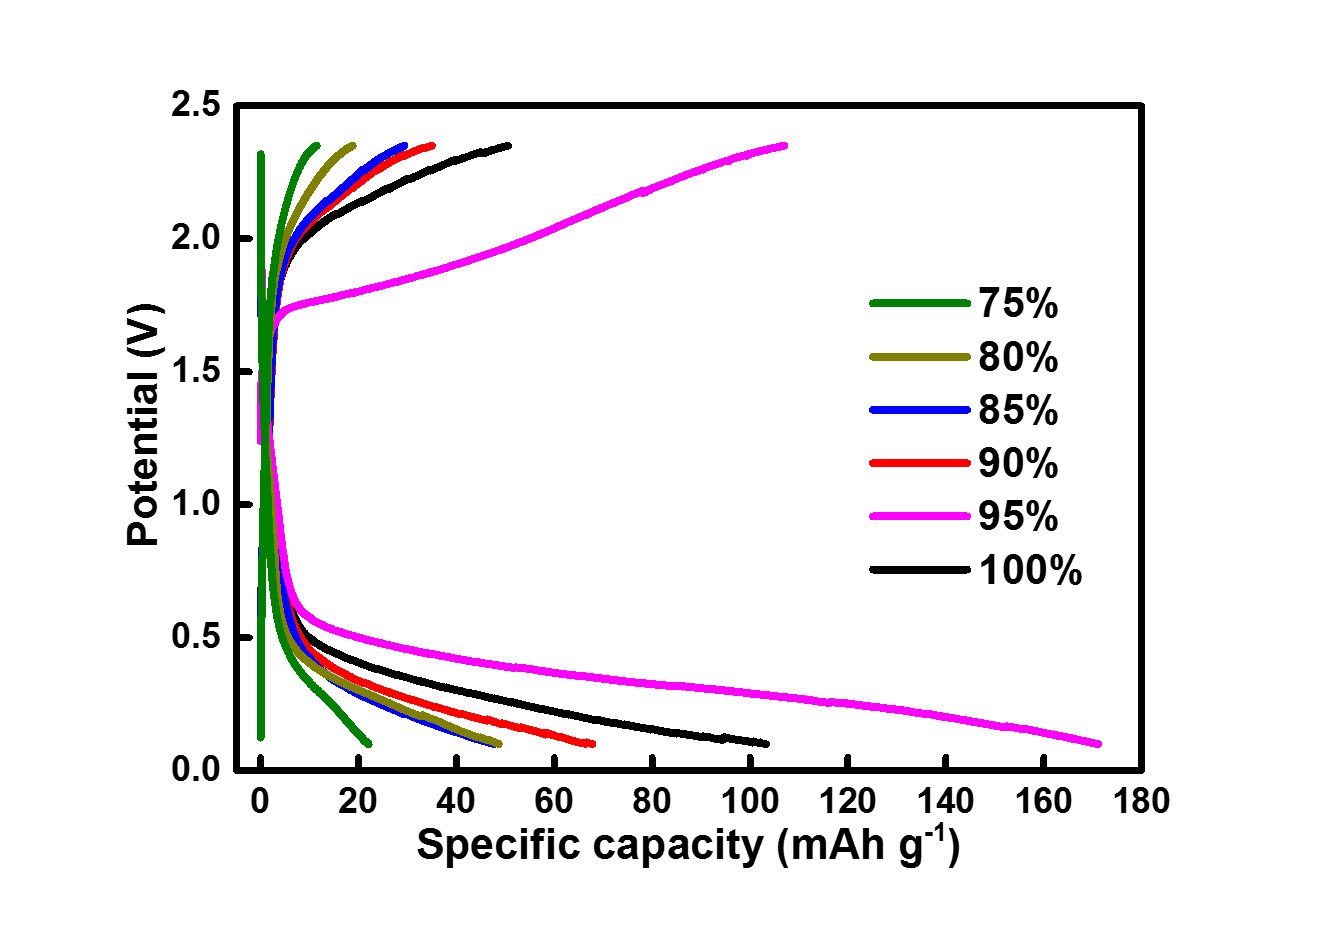
\includegraphics[width=\textwidth]{Figures/BOhBN/hBNBOdifpc}
\caption{Charge/discharge curves of aluminium-ion cells with \ce{B2O3}/hBN as cathode in their 20$^{th}$ cycle. The weight percentage varied from 75\%\ce{B2O3}-25\%hBN to 100\% pure\ce{B2O3}.}
\label{Figures/BOhBN:hBNdifpc}
\end{figure}

Interestingly, it turned out that ratio of 50\% hBN/50\%\ce{B2O3} delivered a very stable capacity of >120 mAh g$^{-1}$ after 20 cycles with a coulombic efficiency of $\sim$80\% as shown in Figure \ref{Figures/BOhBN:hBNBO5050}.

\begin{figure}[tbh!]
\centering
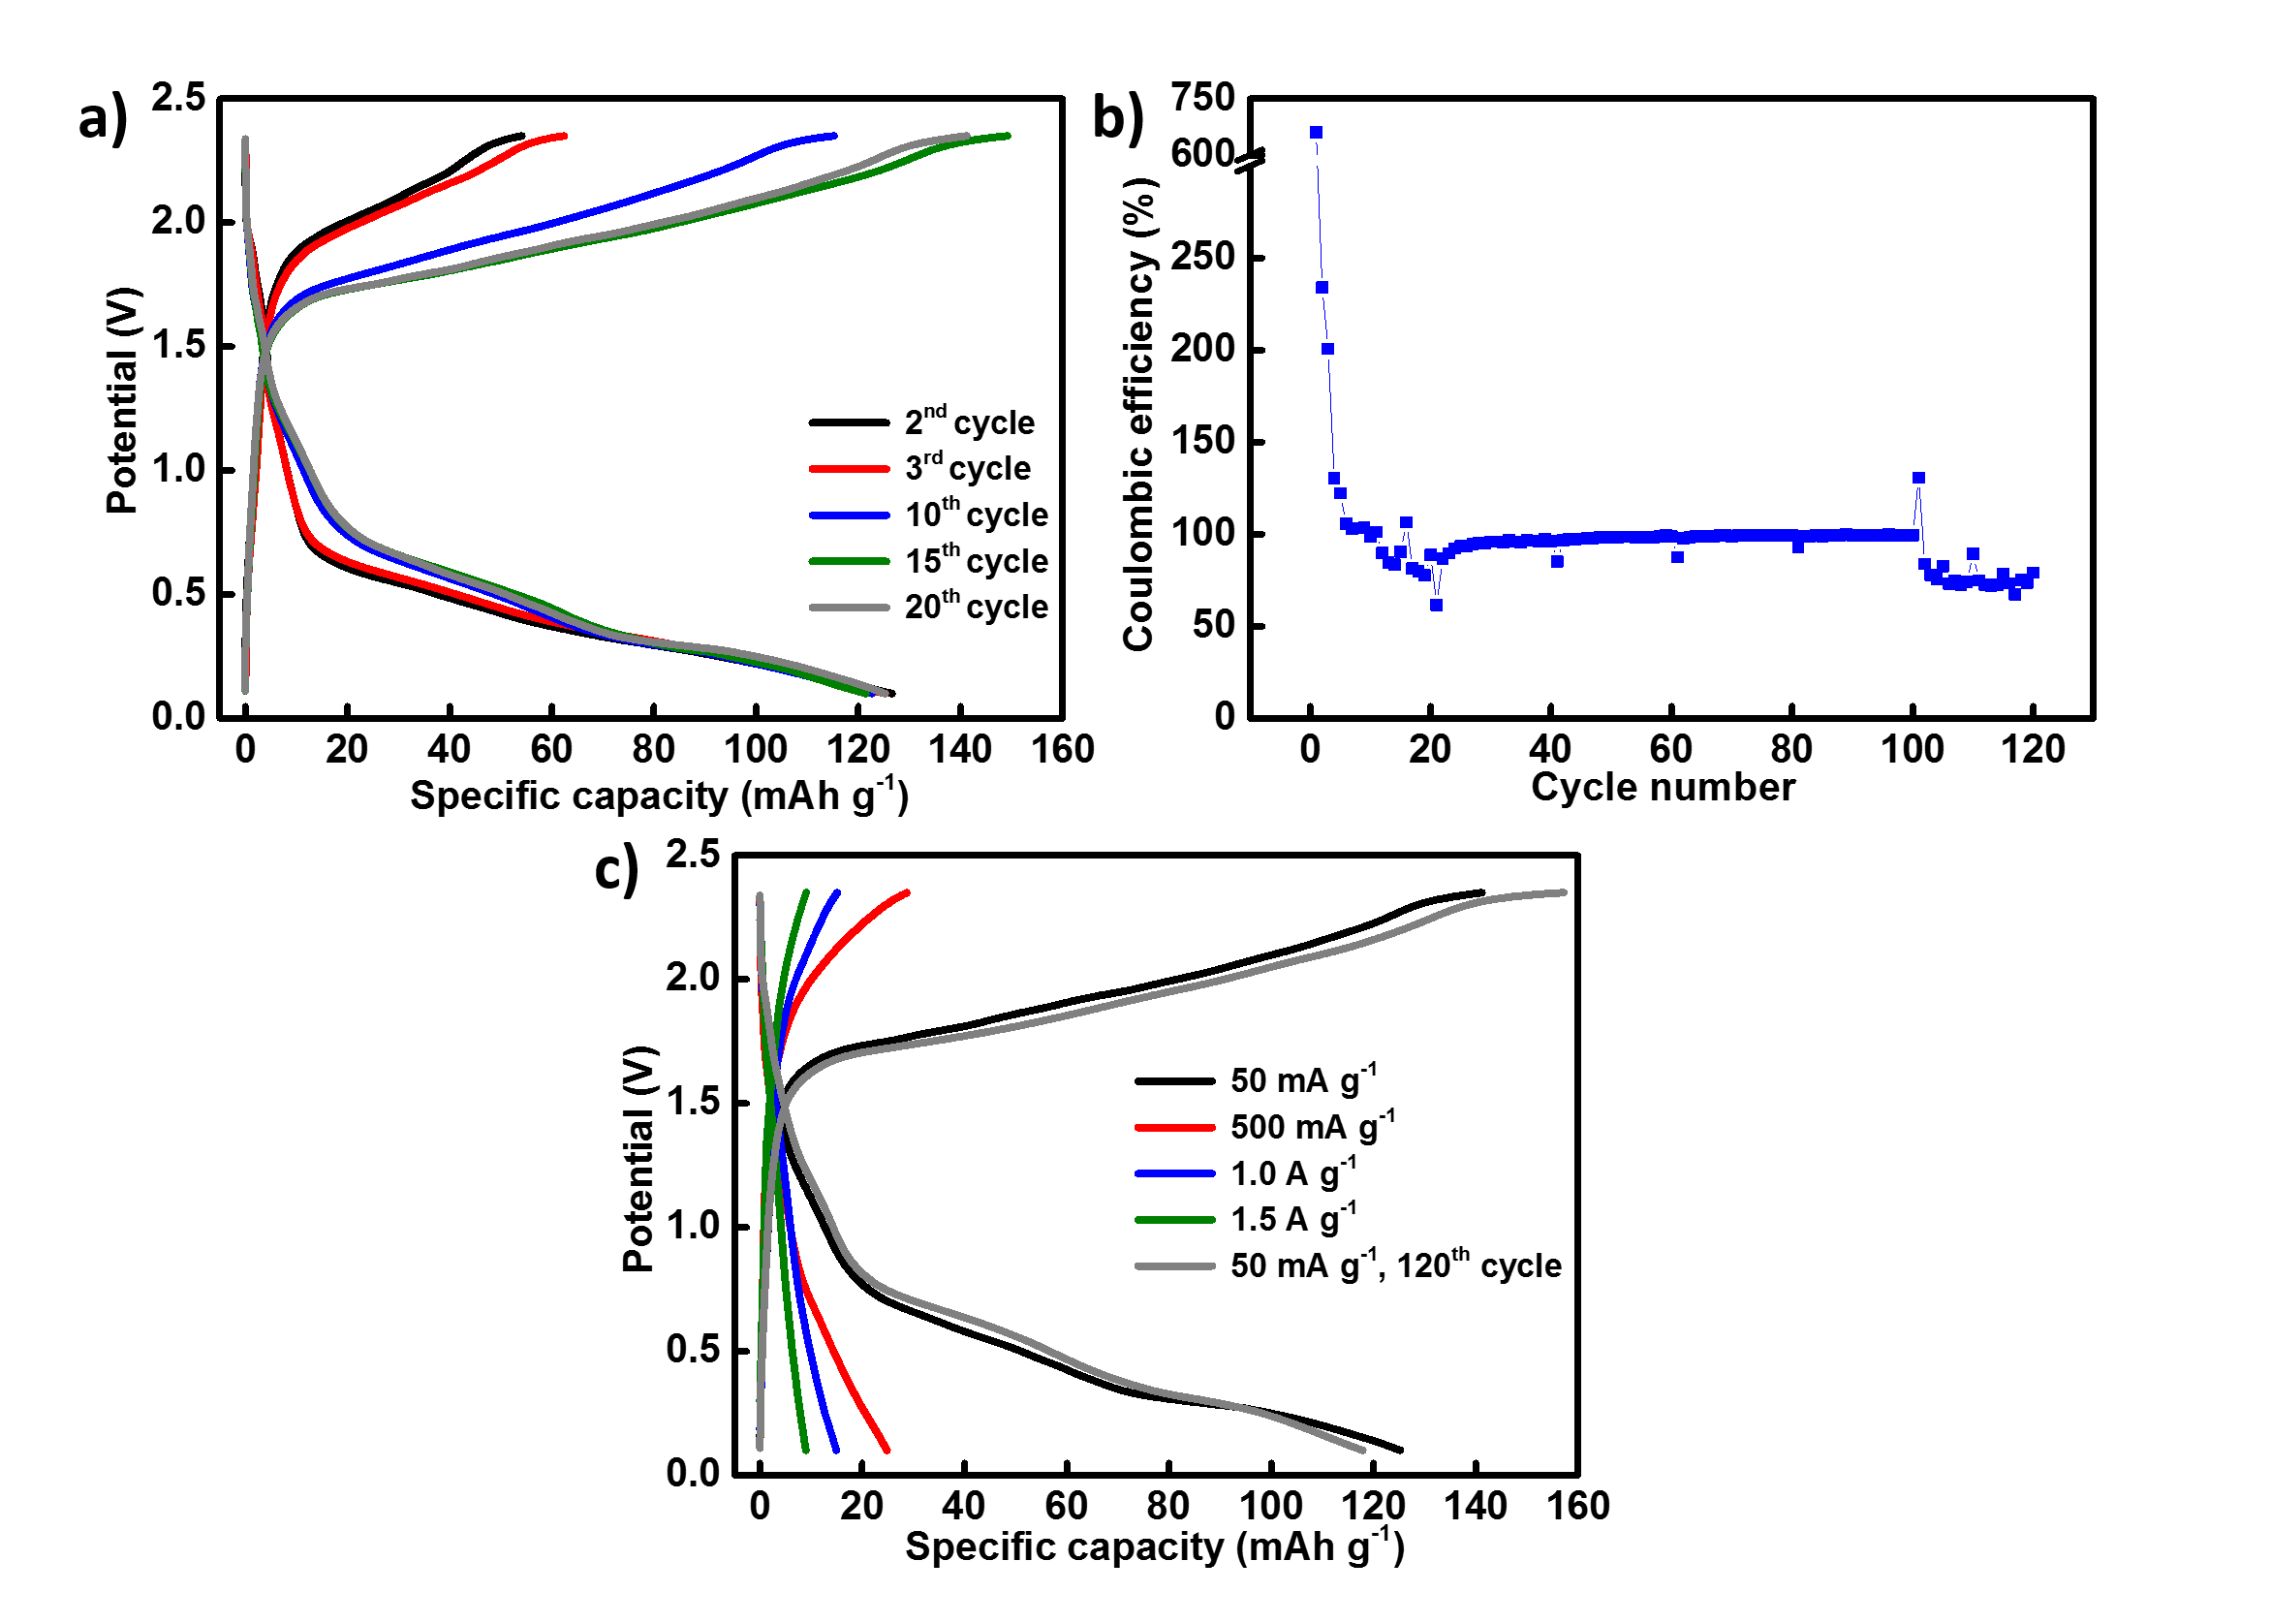
\includegraphics[width=\textwidth]{Figures/BOhBN/hBNBO5050}
\caption{Charge/discharge curves of hBN/ \ce{B2O3} cells a) for the first 20 cycles at a current rate of 50 mA g$^{-1}$, b) coulombic efficiencies and c) long term cell performance at various current densities ranging from 50 mA g$^{-1}$ to 1500 mA g$^{-1}$ .}
\label{Figures/BOhBN:hBNBO5050}
\end{figure}

In order to work out the role of hBN, other nitrides such as graphitic carbon nitride g-\ce{C3N4}, aluminium nitride (AlN) and silicon nitride (\ce{Si3N4}) in a ratio of 1:1, displayed in Figure \ref{Figures/BOhBN:Bonit}. 
\begin{figure}[tbh!]
\centering
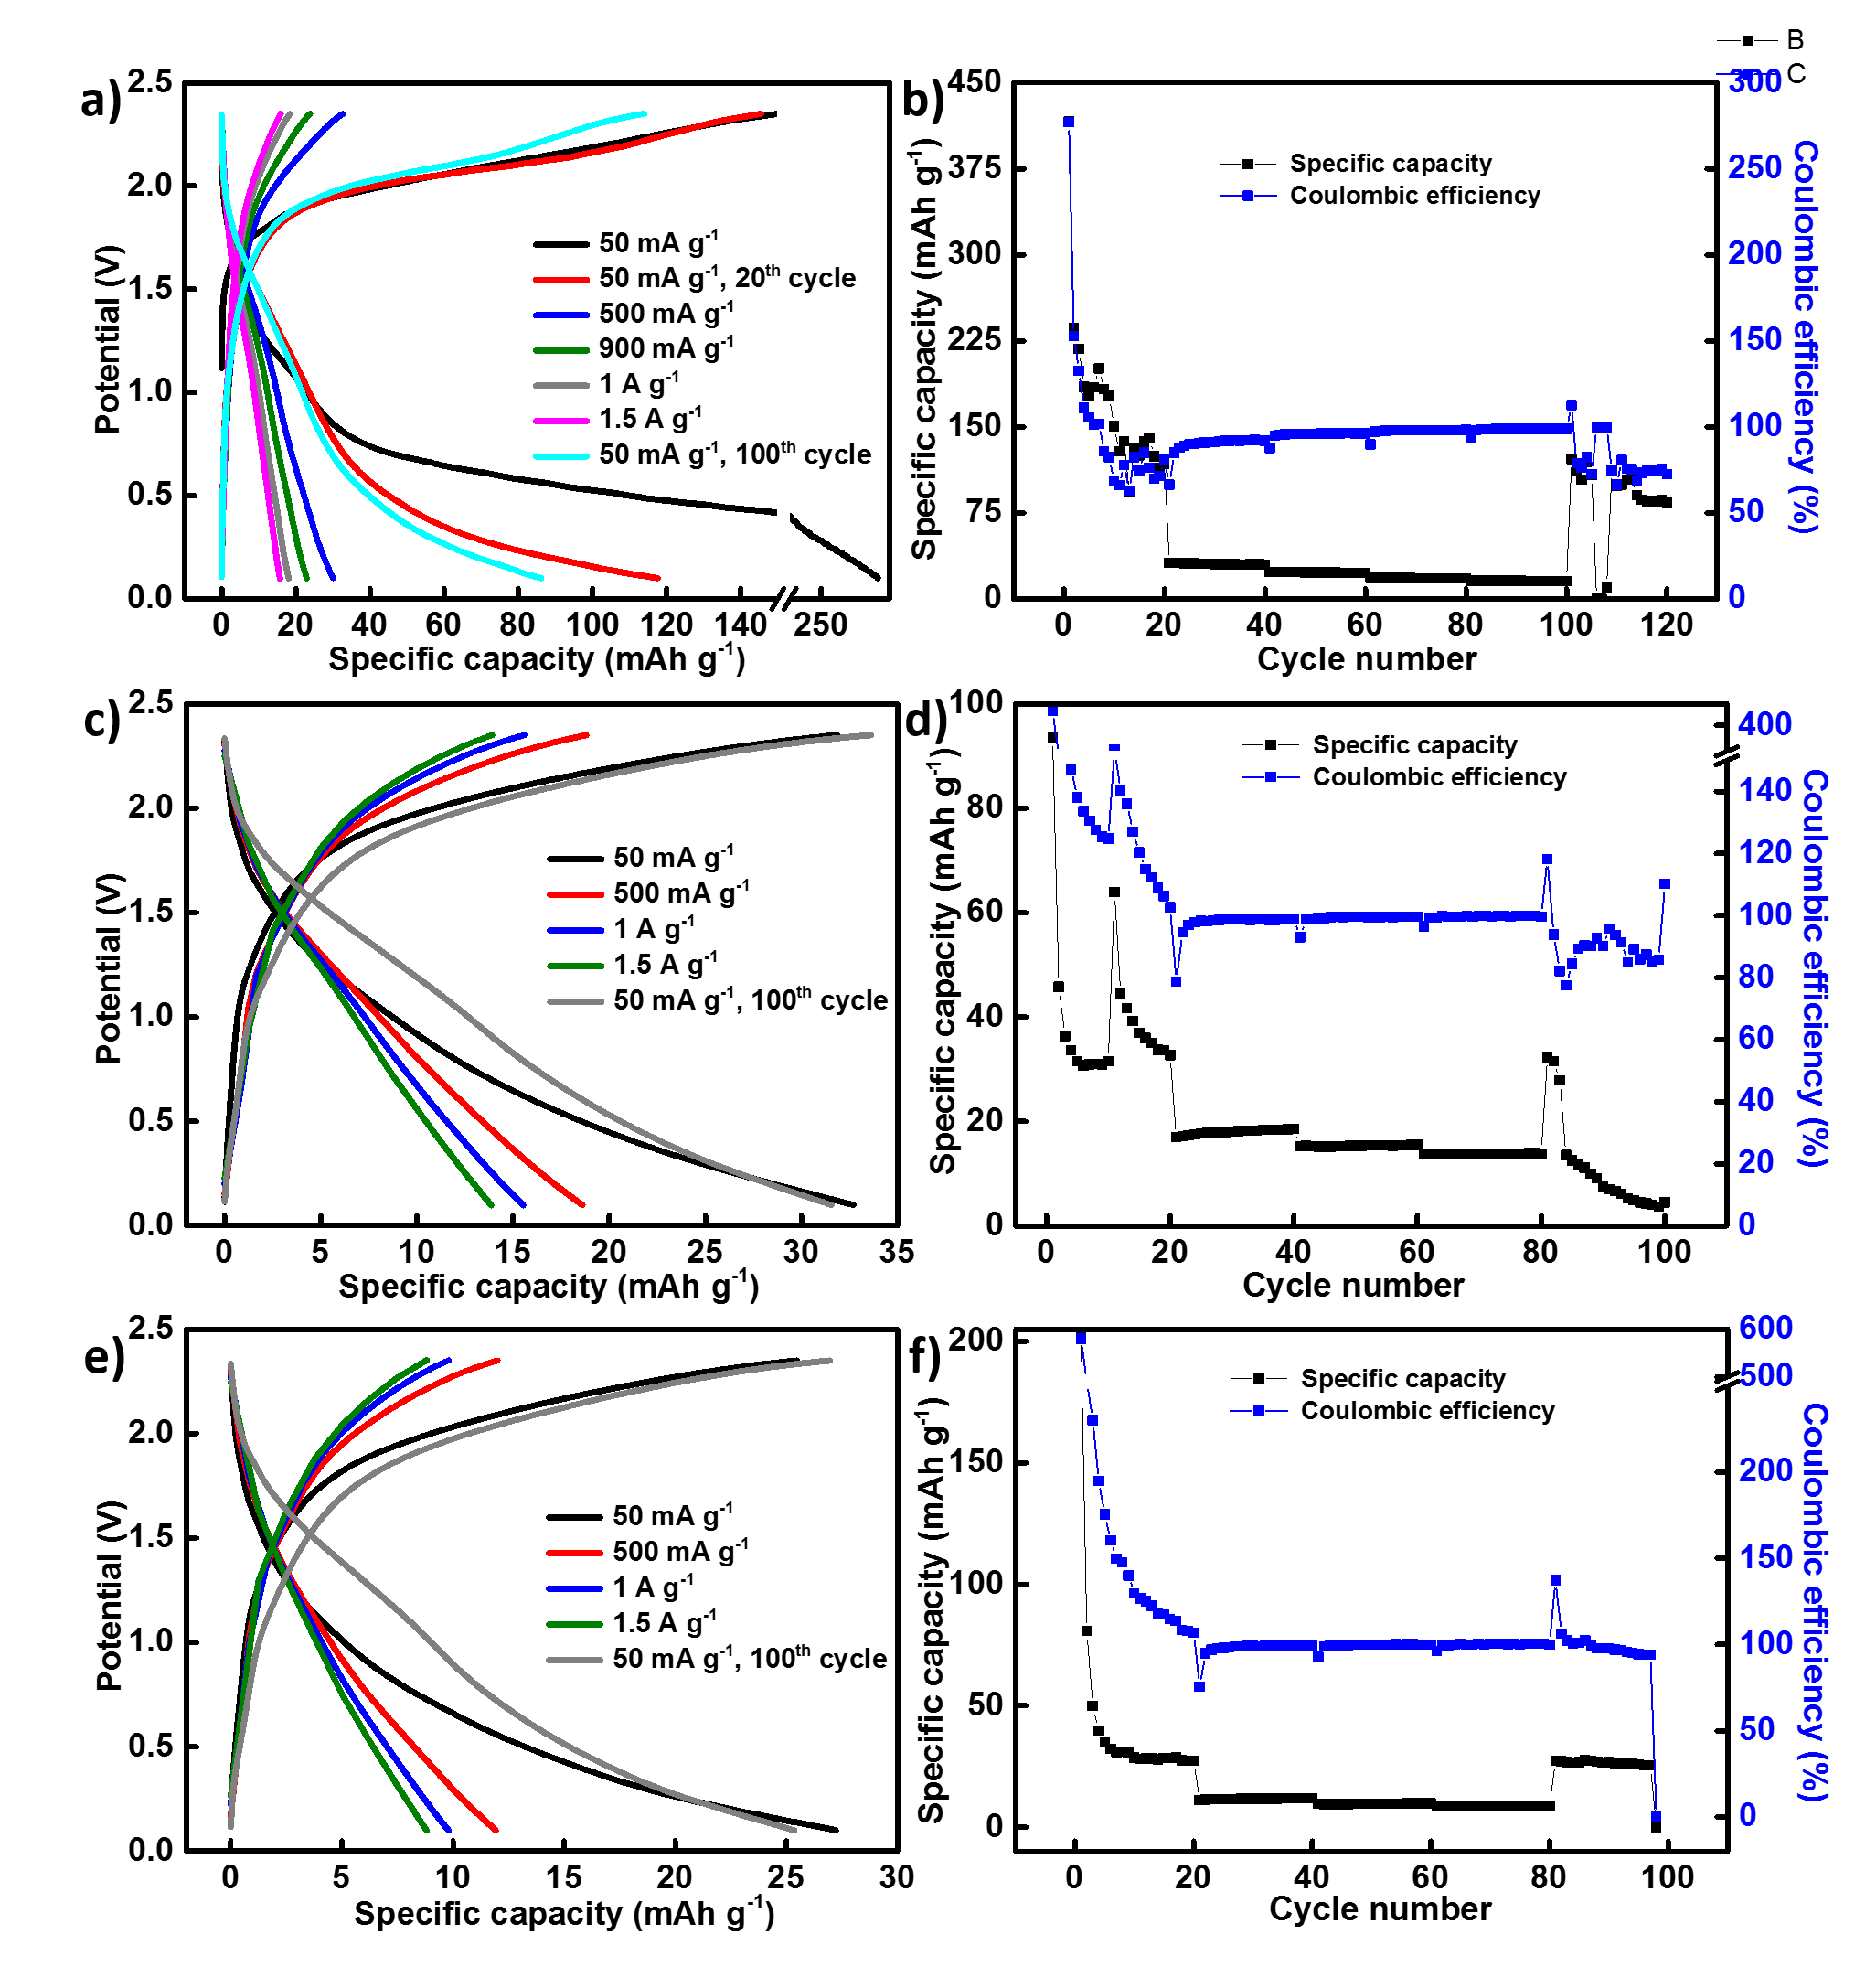
\includegraphics[width=\textwidth]{Figures/BOhBN/Bonit}
\caption{Galvanostatic charge/discharge cycles of cells at different current rates using \ce{B2O3} mixed with other nitrides such as a) \ce{C3N4}, c) AlN and e) \ce{Si3N4} as cathodes. Coulombic efficiencies of b) \ce{B2O3}/\ce{C3N4}, d) \ce{B2O3}/AlN and f) \ce{B2O3}/\ce{Si3N4} cells .}
\label{Figures/BOhBN:Bonit}
\end{figure}

To deduce the role of boric anhydride, other oxides such as manganese dioxide (\ce{MnO2}) and titanium dioxide (\ce{TiO2}) were combined with hBN and tested as cathodes for AIBs. The results are displayed in Figure \ref{Figures/BOhBN:othON}

\begin{figure}[tbh!]
\centering
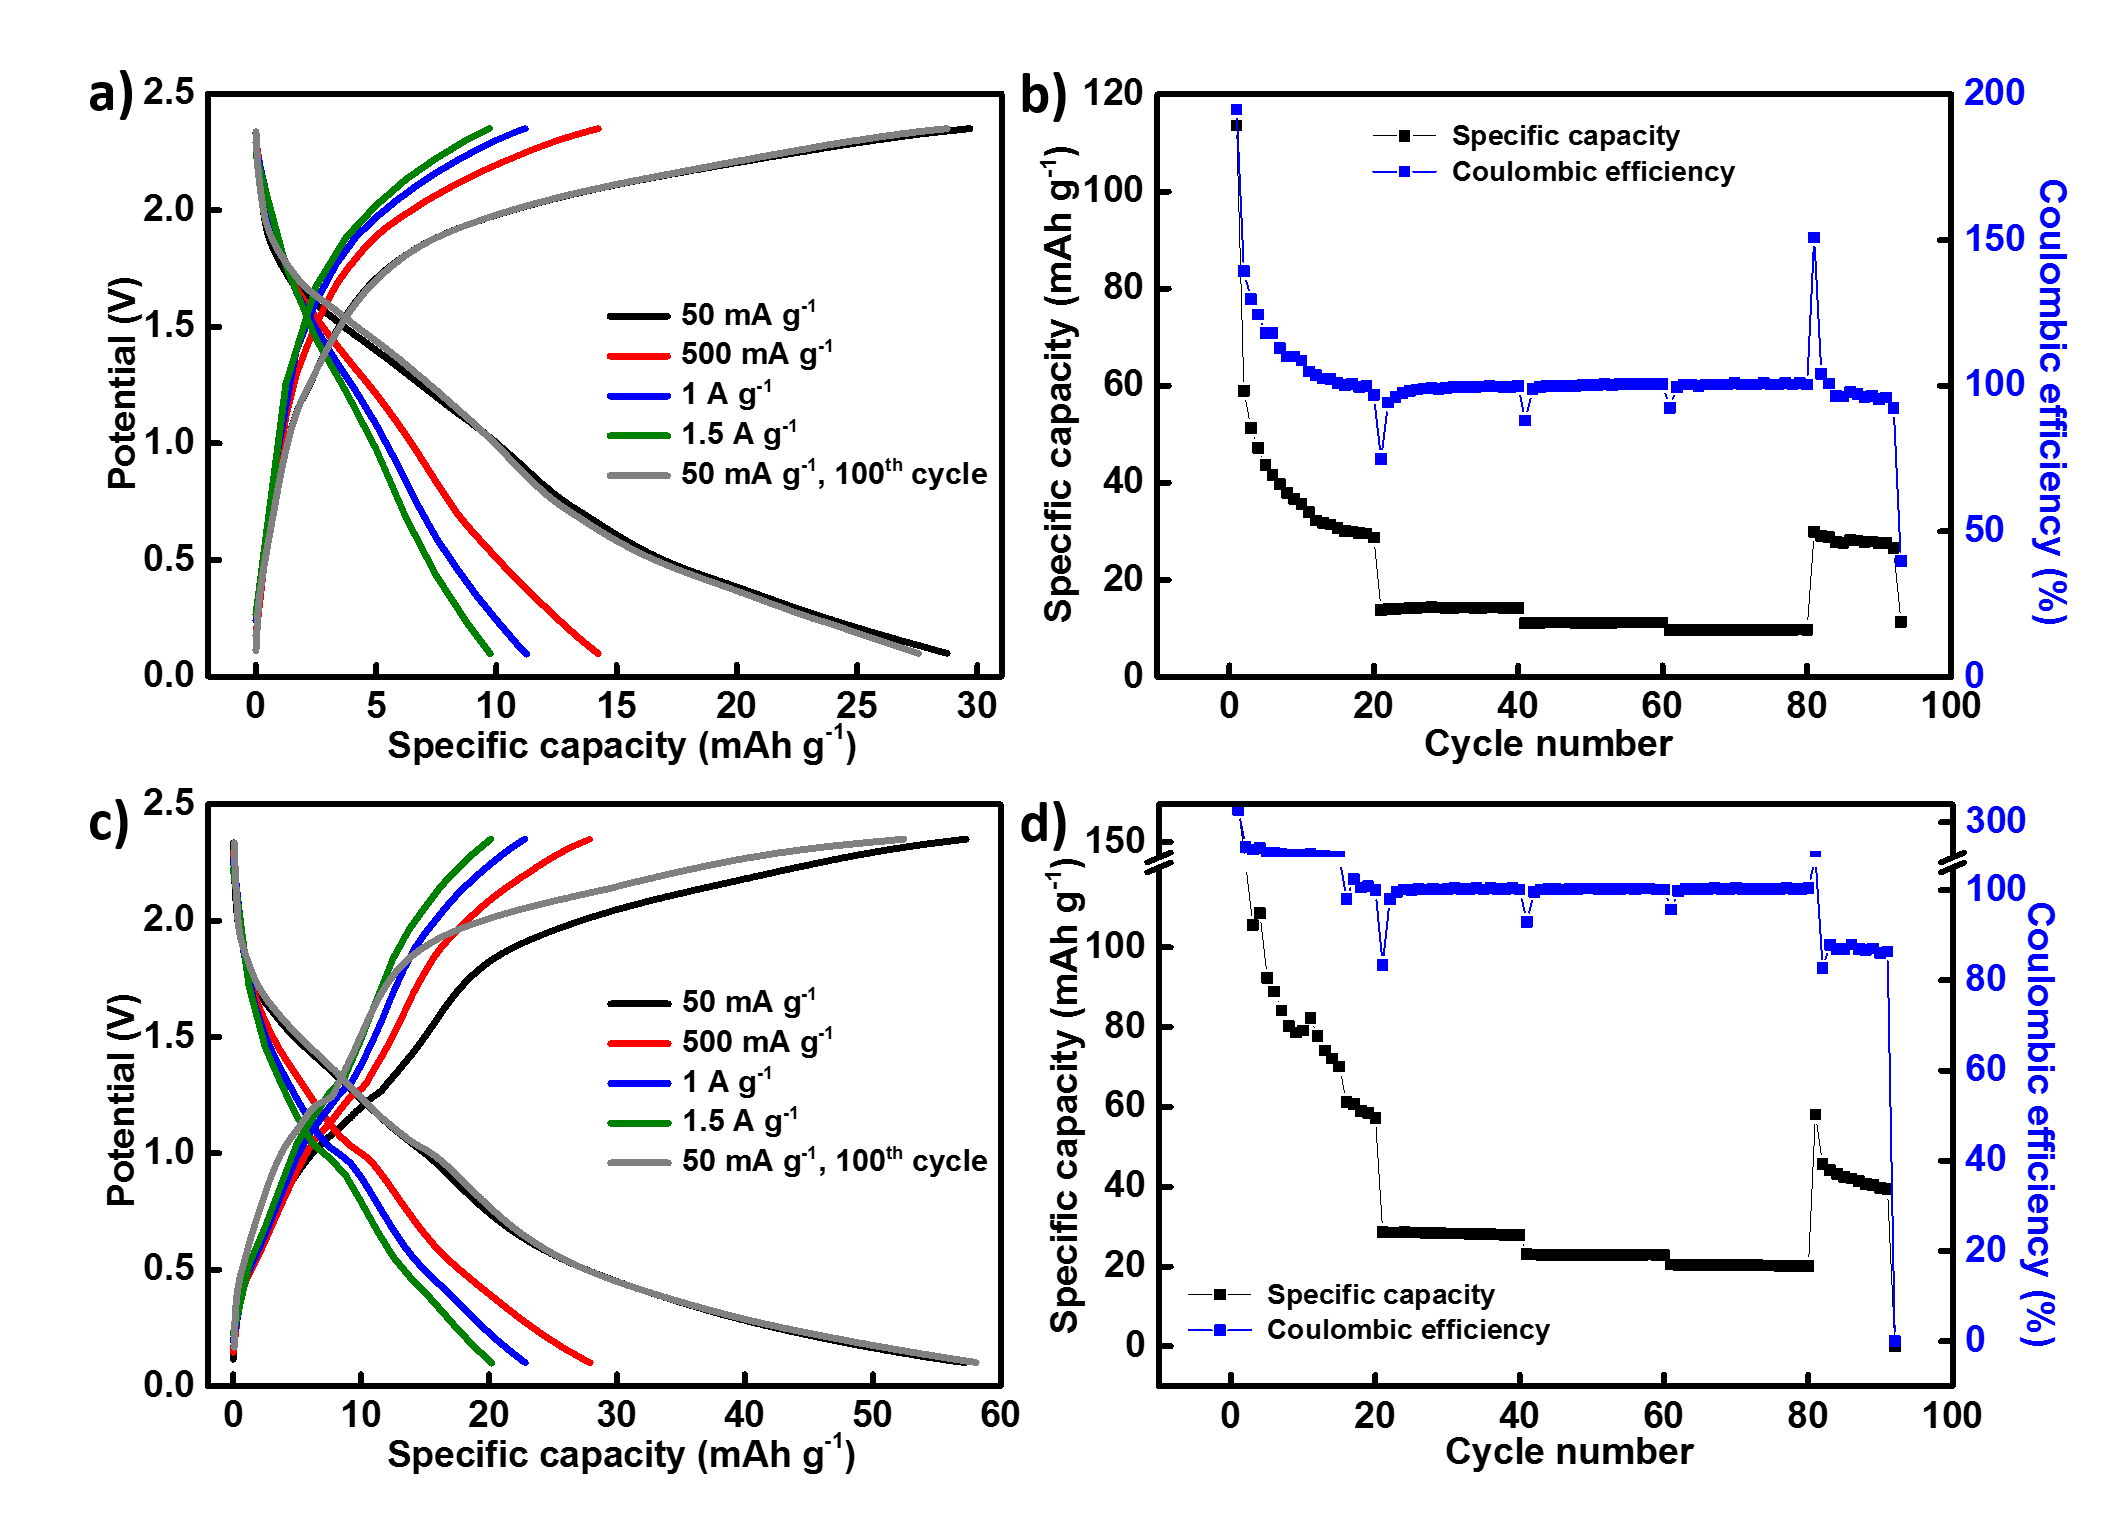
\includegraphics[width=\textwidth]{Figures/BOhBN/BNdifO}
\caption{Galvanostatic charge/discharge profile and cell efficiencies of AIBs composed of a-b) \ce{hBN}/\ce{MnO2} and c-d) \ce{TiO2}/hBN cathodes.}
\label{Figures/BOhBN:BNdifO}
\end{figure}

A few other combinations were tested as cathodes and are displayed in Figure \ref{Figures/BOhBN:othON}.

\begin{figure}[tbh!]
\centering
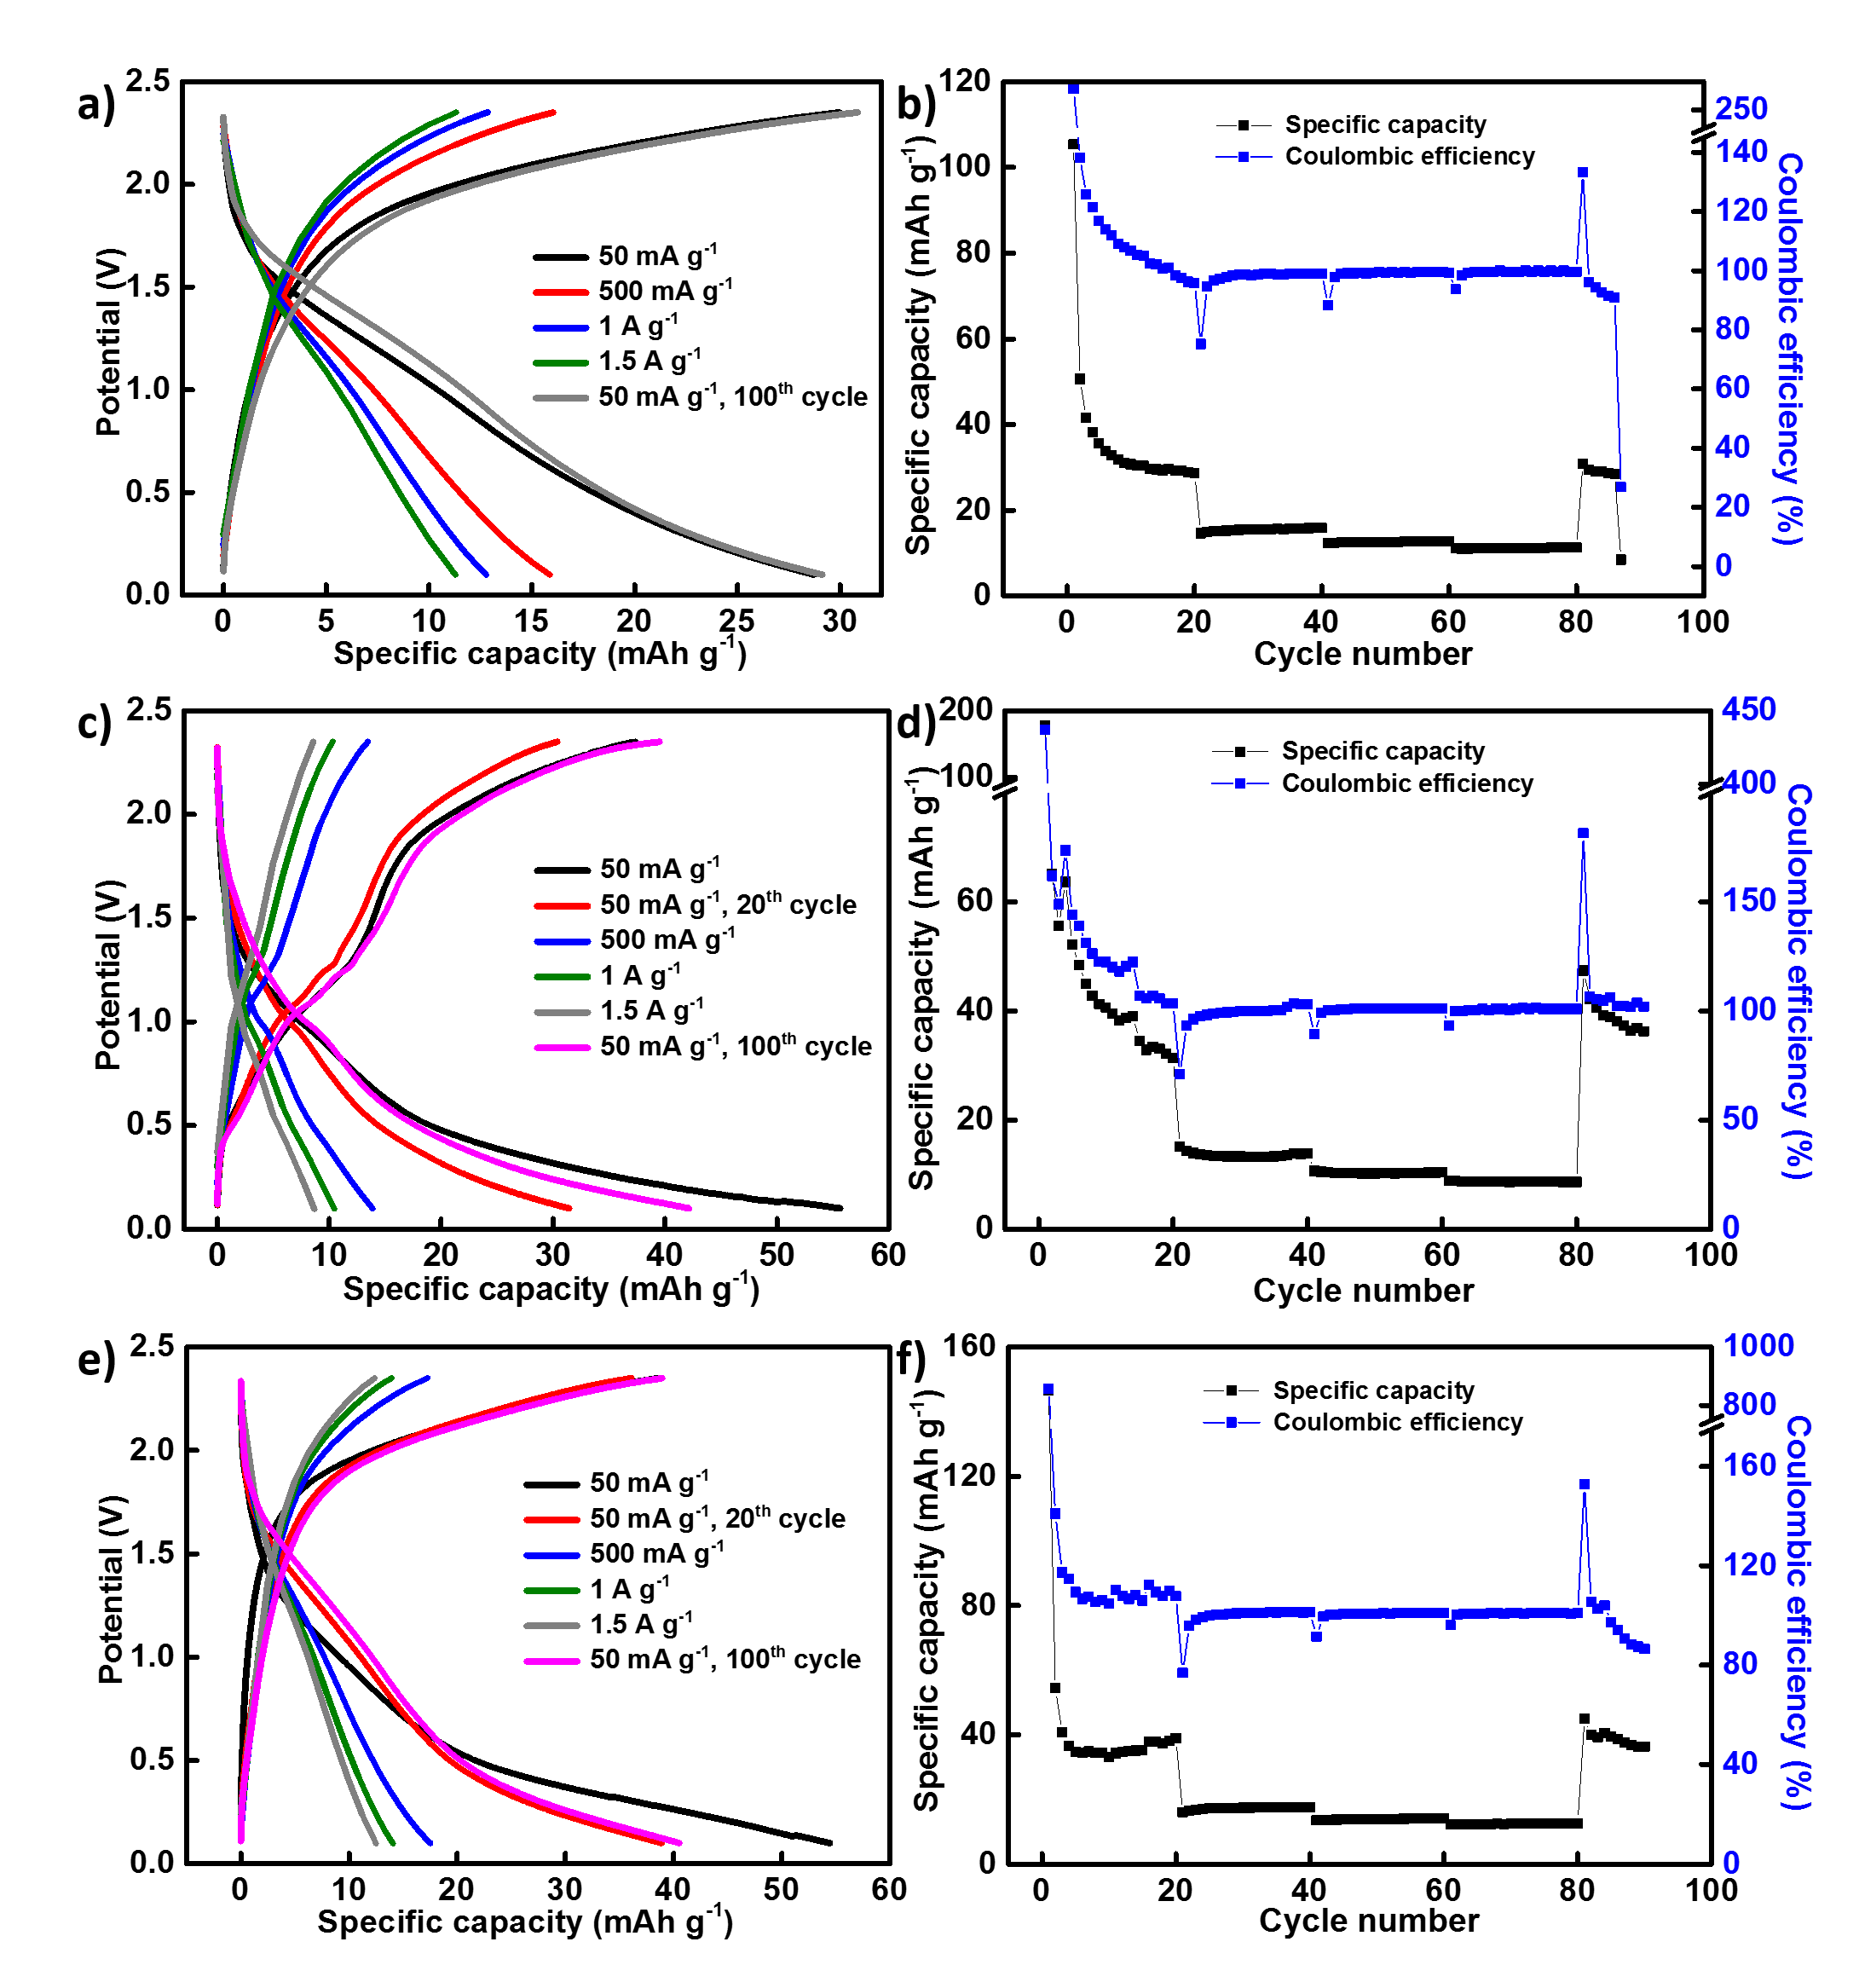
\includegraphics[width=\textwidth]{Figures/BOhBN/othON}
\caption{Galvanostatic charge/discharge profile and cell efficiencies of AIBs composed of a-b) \ce{MnO2}/\ce{C3N4} c-d) \ce{TiO2}/\ce{C3N4} and e-f) \ce{MnO2}/\ce{Si3N4} cells.}
\label{Figures/BOhBN:othON}
\end{figure}

\section{Experimental methods}
Same as described in previous chapters.

